% Compile with xelatex (the Chinese text needs xeCJK and a CJK font). Figures are the vector PDFs in
% paper/figures/out; the references are already formatted (citeproc), so no BibTeX run is needed.
% Options for packages loaded elsewhere
\PassOptionsToPackage{unicode}{hyperref}
\PassOptionsToPackage{hyphens}{url}
\PassOptionsToPackage{space}{xeCJK}
%
\documentclass[
]{article}
\usepackage{amsmath,amssymb}
\usepackage{iftex}
\ifPDFTeX
  \usepackage[T1]{fontenc}
  \usepackage[utf8]{inputenc}
  \usepackage{textcomp} % provide euro and other symbols
\else % if luatex or xetex
  \usepackage{unicode-math} % this also loads fontspec
  \defaultfontfeatures{Scale=MatchLowercase}
  \defaultfontfeatures[\rmfamily]{Ligatures=TeX,Scale=1}
\fi
\usepackage{lmodern}
\ifPDFTeX\else
  % xetex/luatex font selection
  \setmainfont[]{TeX Gyre Termes}
  \ifXeTeX
    \usepackage{xeCJK}
    \setCJKmainfont[]{Noto Serif CJK SC}
          \fi
  \ifLuaTeX
    \usepackage[]{luatexja-fontspec}
    \setmainjfont[]{Noto Serif CJK SC}
  \fi
\fi
% Use upquote if available, for straight quotes in verbatim environments
\IfFileExists{upquote.sty}{\usepackage{upquote}}{}
\IfFileExists{microtype.sty}{% use microtype if available
  \usepackage[]{microtype}
  \UseMicrotypeSet[protrusion]{basicmath} % disable protrusion for tt fonts
}{}
\makeatletter
\@ifundefined{KOMAClassName}{% if non-KOMA class
  \IfFileExists{parskip.sty}{%
    \usepackage{parskip}
  }{% else
    \setlength{\parindent}{0pt}
    \setlength{\parskip}{6pt plus 2pt minus 1pt}}
}{% if KOMA class
  \KOMAoptions{parskip=half}}
\makeatother
\usepackage{xcolor}
\usepackage[margin=2.5cm]{geometry}
\usepackage{longtable,booktabs,array}
\usepackage{calc} % for calculating minipage widths
% Correct order of tables after \paragraph or \subparagraph
\usepackage{etoolbox}
\makeatletter
\patchcmd\longtable{\par}{\if@noskipsec\mbox{}\fi\par}{}{}
\makeatother
% Allow footnotes in longtable head/foot
\IfFileExists{footnotehyper.sty}{\usepackage{footnotehyper}}{\usepackage{footnote}}
\makesavenoteenv{longtable}
\usepackage{graphicx}
\makeatletter
\def\maxwidth{\ifdim\Gin@nat@width>\linewidth\linewidth\else\Gin@nat@width\fi}
\def\maxheight{\ifdim\Gin@nat@height>\textheight\textheight\else\Gin@nat@height\fi}
\makeatother
% Scale images if necessary, so that they will not overflow the page
% margins by default, and it is still possible to overwrite the defaults
% using explicit options in \includegraphics[width, height, ...]{}
\setkeys{Gin}{width=\maxwidth,height=\maxheight,keepaspectratio}
% Set default figure placement to htbp
\makeatletter
\def\fps@figure{htbp}
\makeatother
\setlength{\emergencystretch}{3em} % prevent overfull lines
\providecommand{\tightlist}{%
  \setlength{\itemsep}{0pt}\setlength{\parskip}{0pt}}
\setcounter{secnumdepth}{-\maxdimen} % remove section numbering
\ifLuaTeX
  \usepackage{selnolig}  % disable illegal ligatures
\fi
\IfFileExists{bookmark.sty}{\usepackage{bookmark}}{\usepackage{hyperref}}
\IfFileExists{xurl.sty}{\usepackage{xurl}}{} % add URL line breaks if available
\urlstyle{same}
\hypersetup{
  pdftitle={Supplementary Information},
  hidelinks,
  pdfcreator={LaTeX via pandoc}}

\title{Supplementary Information}
\usepackage{etoolbox}
\makeatletter
\providecommand{\subtitle}[1]{% add subtitle to \maketitle
  \apptocmd{\@title}{\par {\large #1 \par}}{}{}
}
\makeatother
\subtitle{TaoChronos: A Reliable Agent for Knowledge Discovery in
Traditional Chinese Medicine}
\author{}
\date{}

\begin{document}
\maketitle

\textbf{TaoChronos (道乃久)}

Contents: Supplementary Notes 1--4; Supplementary Tables 1--12 (each
also as CSV in \texttt{tables/}); Supplementary Fig. 1; Supplementary
Data 1 (the Discovery Report of the end-to-end run) and 2 (its event
log).

\hypertarget{supplementary-note-1-evaluation-design}{%
\subsection{Supplementary Note 1 \textbar{} Evaluation
design}\label{supplementary-note-1-evaluation-design}}

TaoChronos-Eval has forty suites in three layers. The first tests the
harness's boundaries: nineteen invariants run as probes against the
harness under test, each checked by mutation (the boundary removed, the
invariant broken, the boundary restored; Fig. 4b measures all nineteen
on every variant). The second tests readings: 107 verbatim quotations
that can still be read wrongly, in eight classes, with unsafe errors
(those that would let a false claim through) counted apart. The split
into 23 development and 84 held-out cases was fixed before the suite
first ran, and four blind rounds were each written before the rules that
first read them (Fig. 4d). The third tests research value: a blind
temporal benchmark in which the store is split at a cutoff year,
passages that may have been written on either side belong to neither
side, the rules were written before the first run
(evals/gold/research\_value.yaml) and every read path is bounded in SQL,
so that leakage is counted rather than assumed; graph rankings are
compared with popularity, chance and two other link predictors, and the
pipeline's own predictions are judged by later books.

The other suites measure each capability in the way its task allows:
constructed data where an answer can be constructed (planted drug pairs,
artificial manuscript traditions, a lost work quoted by four books), a
development set where rules need examples, and results the literature
already holds where the real corpus can be checked (the taboo renamings
of Fig. 6, the Yunqi chapters of the Suwen, the first gloss of 几几).
Development and constructed sets were written with the rules they test;
they are regression tests of intended behaviour, and only held-out or
real-corpus results estimate generalization (Supplementary Fig. 2). The
two held-out sets of the V2 layer (entities, ancient phenotypes) were
annotated before the rules ran on them. Everything but the full-corpus
suites reruns on the demonstration corpus in under a minute
(\texttt{taochronos\ eval}); the full-corpus values, which need a store
that is not distributed, are transcribed from docs/evals.md and marked.
Supplementary Table 1 lists every suite.

\textbf{Supplementary Table 1 \textbar{} The forty evaluation suites:
question, data and split, metrics, result and where the paper reports
them} (\texttt{tables/S1\_evaluation\_design.csv})

\begin{longtable}[]{@{}
  >{\raggedright\arraybackslash}p{(\columnwidth - 12\tabcolsep) * \real{0.1429}}
  >{\raggedright\arraybackslash}p{(\columnwidth - 12\tabcolsep) * \real{0.1429}}
  >{\raggedright\arraybackslash}p{(\columnwidth - 12\tabcolsep) * \real{0.1429}}
  >{\raggedright\arraybackslash}p{(\columnwidth - 12\tabcolsep) * \real{0.1429}}
  >{\raggedright\arraybackslash}p{(\columnwidth - 12\tabcolsep) * \real{0.1429}}
  >{\raggedright\arraybackslash}p{(\columnwidth - 12\tabcolsep) * \real{0.1429}}
  >{\raggedright\arraybackslash}p{(\columnwidth - 12\tabcolsep) * \real{0.1429}}@{}}
\toprule\noalign{}
\begin{minipage}[b]{\linewidth}\raggedright
Layer
\end{minipage} & \begin{minipage}[b]{\linewidth}\raggedright
Suite
\end{minipage} & \begin{minipage}[b]{\linewidth}\raggedright
Question
\end{minipage} & \begin{minipage}[b]{\linewidth}\raggedright
Data and split
\end{minipage} & \begin{minipage}[b]{\linewidth}\raggedright
Metrics
\end{minipage} & \begin{minipage}[b]{\linewidth}\raggedright
Result
\end{minipage} & \begin{minipage}[b]{\linewidth}\raggedright
Reported in
\end{minipage} \\
\midrule\noalign{}
\endhead
\bottomrule\noalign{}
\endlastfoot
Boundaries & invariants & Do the harness's boundaries hold --- scope on
every read path, semantic support at commit, objections a model cannot
close, AfterToolCall denials, isolation of model code, atomic batches,
G7 for experts only, evidence bounds, G8 by stance and level, read-only
agent views, integrity, retraction, publication on current versions,
acceptance ≠ execution? & 19 probes (the audit's counterexamples
P01--P10 and nine boundaries added with them) run against the harness
under test; six boundaries removed in turn (mutation) & held / exercised
/ broken & 19/19 held (P01--P10 and nine boundaries added with them);
each of six boundaries removed on purpose (scope guard, result firewall,
semantic support hook, reducer authority, evidence bounds, publish
guard) breaks its invariant & Fig. 4b; Table 2 \\
Readings & interpretive & Are true quotes read right where the reading
is hard --- inverted relations, a prohibition beside a prescription,
consequences, reported and rejected views, omitted conditions, mixed
witnesses, disputed dates, textual cruxes? & 107 verbatim cases in 8
classes (gold/interpretive.yaml); 23 development, 84 held-out, split
fixed before the first run; 4 blind rounds & accuracy and unsafe errors,
per class and per split (dev / held-out) & held-out 82/84 (0.976), 2
unsafe (大黄牡丹汤 read as an indication; 里水, a crux the harvest does
not find); dev 23/23. First blind round 43/53 (0.811); round 3, before
the crux registry, 7/10 with 3 unsafe cruxes; see below & Fig. 4c,d;
Table 2 \\
Research value & research\_value & On the full corpus split at a cutoff
year: do the graph rankings D4 uses anticipate the remedies later books
link to a disease, better than popularity and chance? Do the pipeline's
own predictions, made on the past alone, come true? & full corpus split
at 1127 and 1368: 230 topic--cutoff pairs read, 189 with a link that
came true, 29,467 candidates; the pipeline run on the past view at 1368
for 2 development and 4 held-out topics; replicated on the open corpus
(Supplementary Fig. 3) & hits and precision@k, mean average precision,
paired sign tests over topics; predictions held (strict / loose), per
split and review status; leakage & precision@10 0.168 (popularity 0.134;
chance 0.054); average precision above popularity in 149 of 189 pairs (P
= 2.4 × 10⁻¹⁶); held-out predictions: discoveries 7/19; open corpus:
above popularity 24/6 (P = 0.0014), not separable from chance 13/17 (P =
0.58) & Fig. 5; Supplementary Fig. 3; Table 2 \\
Verification & philology & Are contested readings kept with
probabilities and an uncertain mass? Are variant spellings normalised
for matching? & 7 contested readings (gold/philology.yaml) & pass rate &
7/7 & --- \\
Verification & claims & Does extraction find the right hyperedges
(relation + key arguments + negations)? & 42 gold hyperedges
(gold/claims.yaml), development & precision · recall · F1 · recall by
relation · provenance pass rate & P 1.0 · R 0.976 · F1 0.988 (miss: the
second 湿痹 sign definition). Before the general PROGNOSIS rule (则愈 /
自愈 / 欲解 / 可治 \ldots{} / 者死 / 难治 / 不治 \ldots): P 0.976 · R
0.952 · F1 0.964, prognosis recall 0 --- this gold is dev & Table 2 \\
Verification & provenance & Are all committed claims and evidence
verbatim? How deep is the Claim → Pixel chain? & every claim and
evidence record a demonstration run commits & verbatim rates · chain
depth · level availability & 100\% verbatim claims and evidence; mean
chain depth 7.8; page/line/region/image unavailable (no images in the
demo) & Table 2 \\
Verification & hallucination & Are fabricated, one-character-perturbed
and mis-positioned quotes caught, without flagging real quotes or
variant spellings? & 60 random passages × 4 probes: verbatim, one
character replaced, random characters, shifted span & detection rates ·
verbatim recall & fabricated 100\% · perturbed 100\% · wrong span 100\%
detected; verbatim recall 100\%; variant spelling accepted & Fig. 4a;
Table 2 \\
Verification & contradiction & Contradiction vs conditional vs apparent
vs support vs unrelated (including differential diagnosis and
transcription) & 12 passage pairs (gold/contradictions.yaml) & accuracy
· macro-F1 · confusion & 12/12 & --- \\
Verification & lineage & Formula derivation, citation, transcription,
rephrasing, inheritance, opposition & typed links of the demonstration
corpus (gold/lineage.yaml) & precision (judged) · recall · unjudged
predictions & P 0.867 · R 0.929 --- false positives 逍遥散 ← 苓桂术甘汤
and 补阳还五汤 ← 透脓散 (convergent compositions); miss: 王清任's
implicit opposition & --- \\
Verification & temporal & Period constraints, earliest attestations
(through variant spellings and concepts that predate their names),
period leakage & 6 period constraints, 6 earliest attestations
(gold/temporal.yaml) & accuracies · leakage count & constraints 6/6 ·
earliest 6/6 · leakage 0 & Table 2 \\
Verification & anachronism & Are equations of historical and modern
concepts blocked, careful phrasings allowed, mappings typed
conservatively, agent-asserted equivalence refused? & 10 statements, 8
mappings, agent-asserted equivalences (gold/anachronism.yaml) &
statement accuracy · block P/R · mapping accuracy & statements 10/10 ·
mappings 8/8 · agent equivalence blocked & Table 2 \\
Verification & recovery & After crashes at several points, does resume
reach the identical scientific state? Are reruns and parallel runs
identical? & crashes at 4 points of a run; reruns; parallel against
sequential runs & success rate · replay consistency & 4/4 crash points;
deterministic rerun; parallel = sequential; replay consistent & --- \\
Research value & time\_machine & Research on texts before a cutoff (a
separate harness, nothing later indexed); are its structured predictions
borne out by later texts? & the demonstration corpus split at 1368 (a
separate harness indexes the past only) & decidable predictions ·
accuracy (survived vs other) · leakage · link-prediction baselines & a
passage is on one side of the cutoff only when its whole date range is
(straddling texts are in neither the past corpus nor the checking
future; none at 1368); 3 decidable predictions, 2 held (taboo rename
persisted; lost association stayed absent); failed: the 肾气丸-family
core predicted from two members --- 张景岳's 左/右归丸 dropped
泽泻·牡丹皮·茯苓 & --- \\
Research value & source\_rediscovery & Hold out a cited book: is it
re-inferred as a missing source, dated before its earliest citer? & 3
cited books held out (gold/rediscovery.yaml) & recall@3 · date-bound
consistency & 3/3 re-inferred with consistent date bounds & --- \\
Verification & ablations & Which components carry the results? &
demonstration corpus: 6 terms, 12 passage pairs, the agents' context,
runs without the Skeptic & earliest accuracy without routes ·
contradiction accuracy without sense/philology · G5 inflation without
clusters · Context-OS token reduction · false survivals without the
Skeptic & earliest accuracy: all 1.0 · no sense route 0.67 · BM25 only
0.67; contradiction: no sense resolution 0.83 · no philology 0.92; 1
hypothesis would pass G5 only by counting dependent books; Context OS
−94\% tokens; without the Skeptic 1 rejected hypothesis survives and no
revisions happen & Supplementary Fig. 2c \\
Deep discovery & collation & Are the variants of a known tradition
found, and its stemma, groups and contamination recovered? & 5
artificial traditions copied from the demo corpus down a known stemma
(two branches; one witness copied from both) & unit recall / precision ·
split recall · Robinson--Foulds · group precision · contamination P/R &
variant units: recall 0.998 · precision 0.999; the true split recovered
in every trial (RF 0.33: neighbour-joining resolves the true polytomy
--- three copies made independently from one exemplar --- into an extra
split); top-3 groups all genuine (all groups 0.73); contamination P 1.0
· R 1.0 & Table 2 \\
Deep discovery & reuse & Is each reuse typed right (直接引用 \ldots{}
套语相似), and are real reuses found? & 33 author-constructed pairs
(gold/reuse.yaml), all eight types and unrelated pairs & accuracy ·
macro-F1 · mode accuracy · detection P/R/F1 · pipeline recall & accuracy
0.97 · macro-F1 0.965 · mode 0.97; detection P 1.0 · R 0.96 · F1 0.98;
the demo corpus's gold transcriptions and rephrasings found by
study.reuse: 1.0 & Table 2 \\
Deep discovery & stratigraphy & Are the layers of composite texts found,
with their boundaries, and are texts attributed to their authors? & 5
composites of 16 000 characters with blocks rewritten in a second
author's function characters; the real 素问 and 伤寒论 & layer accuracy
· change-point and boundary P/R · attribution accuracy · real checks
(素问 运气七篇, 叔和 chapters) & layer accuracy 0.955; boundaries R 0.90
· P 0.93; change points R 0.37 · P 1.0; attribution 0.89 · real: the
运气七篇 7/7 in the minor layer, both of their boundaries found, 3 of
the 4 chapters flagged by late vocabulary are 运气 chapters, 辨脉法 and
平脉法 nearest the 脉经 & Table 2 \\
Deep discovery & cases & Are case records cut into cases and visits, and
are their fields read right? & 6 constructed cases in the two manners of
the literature --- visits under a heading, narratives (gold/cases.yaml);
the two transcriptions of 吴鞠通医案 & segmentation · per-field accuracy
· response and outcome accuracy · agreement of two transcriptions &
segmentation, fields, responses, outcomes 1.0 on the development set ·
real: case counts agree 0.98, outcomes 0.92 & --- \\
Deep discovery & argument & Are the steps of reasoning found and typed?
& 18 author-constructed passages (gold/argument.yaml); the 脉经's two
transcriptions against 温病条辨 & labelled and unlabelled edge P/R/F1 ·
clause segmentation · same-work vs other-work divergence & edges F1 1.0
on the development set · real: JSD 0.020 between the transcriptions of
one work, 0.091 against another & --- \\
Deep discovery & senses & Is a planted shift of senses dated, and a
sense no cue names found? & synthetic occurrences: one sense rises from
15 \% to 75 \% in the year 1000, an uncued sense appears from 1300 &
change-year error · detection · labelling accuracy · hidden sense found
· curated exemplars & change year within 2.3 years; detected 1.0;
labelling 0.93; the uncued sense found 1.0 (precision 1.0); curated
exemplars of 消渴 6/8 & --- \\
Deep discovery & fragments & Is a lost text rebuilt from its quotations
without taking in other sources' words? & a constructed lost work
(集古方, held out) quoted by four books in the manners of the 外台秘要,
the 医心方, the 证类本草 and a late paraphrase, beside other sources
(gold/fragments/); the real 千金 and 肘后 & precision · coverage · decoy
leaks · volume accuracy · real verification (千金, 肘后) & precision
0.86 · coverage 1.0 · no other source's words taken in · volumes 1.0 ·
real: 千金 precision 0.32 · coverage 0.12; 0.876 of the 肘后's
quotations not in the extant text & Supplementary Fig. 2a; Table 2 \\
Task specification & punctuation & Are the marks of 白文 placed where
editors place them, with every character kept? & the store's punctuated
texts; 55 works held out of training (104 k characters); 4 Siku 白文
works against their 笈成 punctuation & boundary / sentence F1 ·
mark-type accuracy · preservation rate · rule baseline · held-out works
· Siku 白文 & held-out boundary F1 0.767 (P 0.725 · R 0.814; rules
0.235), typed sentence F1 0.543, mark types 0.805; 白文 boundary F1
0.780 (rules 0.303); characters preserved 1.0 & Supplementary Fig. 2b;
Table 2 \\
Task specification & commentaries & Are the commentaries on a clause
found in every layout, attributed and compared? & a constructed classic
with commentaries in four layouts (gold/commentaries/); the real
太阳之为病 & unit P/R/F1 · text F1 · relation F1 · quotation recall ·
real: known commentators and relations & units F1 1.0 · text F1 0.81 ·
relations F1 1.0 · quotations 1.0 · real: 25 commentaries, known
commentators 11/11, 张卿子 照录 成无己 and 喻昌 承袭 方有执 found &
--- \\
Task specification & disputes & Are named views read as rejected or
endorsed, and quoted words kept apart? & 22 author-constructed sentences
(gold/disputes.yaml) & accuracy · reject / endorse P/R/F1 · real: known
controversies & accuracy 0.86 · reject P 1.0 R 0.78 · endorse P 0.8 R
1.0 · real: 3/3 known controversies (景岳 on 丹溪's 相火, 越人's
左肾右命门 \ldots) & --- \\
Task specification & variant\_impact & Is each variant reading classed
by what it changes (dose, negation, drug, finding \ldots)? & 30 readings
(gold/variant\_impact.yaml) & accuracy · macro-F1 · high-impact P/R/F1 ·
real: the review queue of the 伤寒论 & accuracy 0.97 · macro-F1 0.97 ·
high impact P 1.0 R 0.94 · real: the 伤寒论's 288 units, the top 10 of
its review queue all high-impact & --- \\
Task specification & clause & Are the parts of a clause (condition
\ldots{} prognosis) found? & 16 clauses of the 伤寒论 and 金匮
(gold/clause.yaml) & piece accuracy · macro-F1 · per-role F1 ·
segmentation · real: forms of the 伤寒论 & pieces 0.977 · macro-F1 0.92
· real: 40 \% of the pieces of the fullest 伤寒论 witness read by no
rule (平脉法 dialogues, numbering, notes) & --- \\
Task specification & glosses & Are the glosses of a word found, and only
of that word? & 16 sentences (gold/glosses.yaml) & accuracy · P/R/F1 ·
real: the first gloss of 几几 & accuracy 1.0 · P/R 1.0 · real: 成无己's
伸颈之貌 the first gloss of 几几 & --- \\
Task specification & pairs & Do planted drug pairs come first, and do
few chance pairs pass Benjamini--Hochberg? & 600 synthetic compositions
with three planted pairs; the store's 66 196 compositions & planted
top-3 · false significant · real: textbook pairs · 方证 links of 桂枝汤
and 麻黄汤 & planted top-3 1.0 · false significant 0.0 · real: 7/7
textbook pairs significant with lift \textgreater{} 1.5 (桂枝---芍药
2527 compositions, lift 2.05; 麻黄---杏仁 5.08 \ldots) & Fig. 6d; Table
2 \\
Task specification & schools & Are a school's planted words found, and
do the textbooks' doctrines come out as its own? & 5 synthetic 温病
physicians and 16 other authors; the store's schools with the textbooks'
doctrines (gold/schools.yaml, 44) & planted top-2 and significant ·
common words listed · citation shares · real: doctrine recall and
attribution & planted words top-2 and significant, no common word listed
· real: doctrine recall 0.73 (z ≥ 1.96), attribution 0.64 & --- \\
Task specification & names & Is the change of a drug's preferred name
dated, and its names equated and completed? & 20 synthetic works (薯蓣 →
山药); the dated taboo renames (gold/names.yaml) & switch interval ·
nested names apart · equations · candidates · real: dated taboo renames
& switch interval, nested names, equation, candidate 山芋 all right ·
real: 2/2 (薯蓣→山药 in 1000--1200, 玄参→元参 in 1600--1800) & Fig.
6a,b \\
Task specification & chain & Does each witness of a passage hang from
the witness it was copied from? & 6 artificial traditions of 12
witnesses; with each copy regularising spellings on its own & witnesses
found · parent accuracy against the most-similar baseline, with and
without convergent spellings & parent accuracy 1.0 (most-similar
baseline 0.97); with convergent spellings 0.94 (baseline 0.87);
witnesses found 0.96--1.0 & --- \\
V2 & entities & Are the entities of a sentence found and typed (24
types)? & 41 dev sentences, 160 entities (gold/ner.yaml); 25 held-out
sentences, 117 entities, annotated after the rules were written
(gold/ner\_heldout.yaml) & precision · recall · F1 & dev F1 0.991 ·
held-out F1 0.776 (P 0.783 · R 0.769) & Supplementary Fig. 2a; Table
2 \\
V2 & places & Are physicians placed from their signatures, prefaces and
biographies? & 15 signatures and 5 statements of native place in the
forms of real prefaces and biographies, with traps (gold/places.yaml);
the full corpus & precision · recall & P/R 1.0 · 84.6 \% of physicians
placed · real: 291 of 761 works placed, curated places confirmed 4/4,
湿温 in 清 江南 49 \% vs 26 \% (q 0.108, not significant) & --- \\
V2 & translation & Does a translation keep the original layer and add no
present-day diagnosis? & 24 presentism cases (equations, retrospective
diagnoses, modern names a translation adds, comparisons that must pass);
the demo corpus & guard accuracy · layer preserved & guard 24/24 ·
original layer unchanged 24/24 · doublets glossed by their commentators
3/3 & --- \\
V2 & layout & Are page images read in order, with notes, margins and OCR
errors located? & 60 synthetic pages (vertical, 双行小注, 版心, 书眉;
noisy and character-level variants); four OCR formats; 12 OCR texts with
one error each & reading-order accuracy · CER · notes F1 & reading order
exact 0.983 · CER 0.0005 · notes F1 0.999 · formats identical · errors
located 12/12 & --- \\
V2 & bridge & Are the findings of a passage projected into HPO with
typed relations? & 20 dev sentences; 12 held-out passages drawn at
random from 65 clinical works of the full corpus, annotated before the
reader ran on them; 18 canonical descriptions and 2 negatives
(gold/bridge.yaml) & precision · recall · F1 & dev F1 0.985 · held-out P
0.938 · R 0.732 · F1 0.822, bounds 1.0 · mapping top-1 1.0, caps 3/3,
guard 20/20 · 213 HPO ids valid in hp/releases/2026-09-01 &
Supplementary Fig. 2a; Table 2 \\
V2 & audit & Does each statement of an answer get the verdict its
evidence supports? & 19 claims of every kind and 3 safety texts
(gold/audit.yaml) & verdict accuracy · false SUPPORTED & verdicts 1.0 ·
kinds 1.0 · false SUPPORTED 0 · safety 3/3 & Table 2 \\
V2 & modern & Are modern records typed by design and population, and
cross-level claims refused? & 10 records to type, 7 claim/evidence pairs
for the cross-level guard, the synthetic OMOP database
(gold/modern.yaml) & typing accuracy · guard accuracy & typing 10/10 ·
guard 7/7 · RWD: SQL checks pass, planted association recovered, bad SQL
refused & --- \\
V2 & workflow & Does the orchestrator plan the skills a question needs
and no others? & the registry; 8 questions with the skills they need and
must not call (gold/workflow.yaml); one end-to-end run & valid plans ·
rerun from the workspace & registry valid · plans 8/8 · a rerun reads
every step from its workspace & --- \\
Verification & aliases & Is a drug found under its other names (国老 for
甘草, 通草 for 木通 before 960) without losing the name asked, merging
two drugs that share a name or reaching outside the years a name meant
the drug? (\protect\hyperlink{alias-layer-aliases}{below}) & & synthetic
checks; per profile, split and item type, for off, naive, on, analysis
and the ablations: P@10 (and its gain where off answers) · nDCG@10 ·
AskedRet@10 (mean, min) · ON@10 · ON@50 · XR@50 · Wrong@10 · CandRecall
· CandPrecision · SilentMerge · FlagP/FlagR · Leakage · latency p50/p95;
resolution accuracy & 9 planted items on a corpus written for the eval:
every check held (side places and retention at k = 5, 10, 20; no merge;
gates; readings; periods; flags; no leakage; off = today's search); P@10
off 0.800 · naive 0.806 · on 0.933; Wrong@10 6 · 7 · 3; on: CandRecall
1.0, SilentMerge 0, FlagR 1.0, leakage 0 & --- \\
\end{longtable}

\hypertarget{supplementary-note-2-gates-permissions-and-authority}{%
\subsection{Supplementary Note 2 \textbar{} Gates, permissions and
authority}\label{supplementary-note-2-gates-permissions-and-authority}}

Five mechanisms bound what any part of the harness can do, and they are
layered so that the failure of one is caught by another (Fig. 4b). (1)
Permissions: every tool needs one permission, and an agent holds only
those its specification lists (Supplementary Tables 4 and 5); an agent
that asks for a tool outside them is refused and the refusal is logged.
(2) Hooks: deterministic guards at eight points of the lifecycle
(Supplementary Table 6) refuse a tool call or result outside the
research's scope, a claim whose quote is not verbatim or contradicts it,
an anachronistic equation and a report on unjudged versions. (3) Event
authority: every change to the research object is an event, and the
reducer refuses an event its principal may not emit; 61 event types,
nine patterns of permission (Fig. 1b, Supplementary Table 7). An agent
proposes; only validators grade, and only a human sets G7. (4) Gates
G0--G8 grade each claim, evidence record and hypothesis on its current
version (Supplementary Table 2). (5) The research contract, hashed
before the first task, fixes the criteria by which a hypothesis is
accepted, needs an expert, stays inconclusive or is rejected, and names
the judge of each (Supplementary Table 3): finishing the tasks never
accepts a research. In conversation, four core agents run the same
specialists as fifteen skills (Supplementary Table 8).

\textbf{Supplementary Table 2 \textbar{} Gates G0--G8: what each passes,
warns and fails, and who sets it} (\texttt{tables/S2\_gates.csv})

\begin{longtable}[]{@{}
  >{\raggedright\arraybackslash}p{(\columnwidth - 12\tabcolsep) * \real{0.1429}}
  >{\raggedright\arraybackslash}p{(\columnwidth - 12\tabcolsep) * \real{0.1429}}
  >{\raggedright\arraybackslash}p{(\columnwidth - 12\tabcolsep) * \real{0.1429}}
  >{\raggedright\arraybackslash}p{(\columnwidth - 12\tabcolsep) * \real{0.1429}}
  >{\raggedright\arraybackslash}p{(\columnwidth - 12\tabcolsep) * \real{0.1429}}
  >{\raggedright\arraybackslash}p{(\columnwidth - 12\tabcolsep) * \real{0.1429}}
  >{\raggedright\arraybackslash}p{(\columnwidth - 12\tabcolsep) * \real{0.1429}}@{}}
\toprule\noalign{}
\begin{minipage}[b]{\linewidth}\raggedright
Gate
\end{minipage} & \begin{minipage}[b]{\linewidth}\raggedright
Name
\end{minipage} & \begin{minipage}[b]{\linewidth}\raggedright
Subject
\end{minipage} & \begin{minipage}[b]{\linewidth}\raggedright
Pass
\end{minipage} & \begin{minipage}[b]{\linewidth}\raggedright
Warn
\end{minipage} & \begin{minipage}[b]{\linewidth}\raggedright
Fail
\end{minipage} & \begin{minipage}[b]{\linewidth}\raggedright
Set by
\end{minipage} \\
\midrule\noalign{}
\endhead
\bottomrule\noalign{}
\endlastfoot
G0 & Source & claim, evidence & the book is in the store with an origin
and a licence (score 0.8 when the transcription is unverified) & --- &
unknown book, or no origin or licence & validator \\
G1 & Transcription & claim, evidence & a verified manual transcription,
or OCR confidence ≥ 0.9 & an unverified transcription, or OCR confidence
0.7--0.9 & OCR confidence \textless{} 0.7 & validator \\
G2 & Philology & claim, evidence & text collated against an edition, and
the span not on a contested reading & uncollated text, or a contested
reading whose base reading has p ≥ 0.4 & the span rests on a contested
reading with p \textless{} 0.4 & validator \\
G3 & Sense & claim; hypothesis & every term resolved to one sense for
its period & a homonym whose most likely sense has p \textless{} 0.6 &
--- & validator \\
G4 & Claim provenance & claim, evidence; hypothesis & the quote is
verbatim at its span and states the relation & verbatim, but the quote
does not clearly state the relation, or states a view the author rejects
& the quote is not verbatim or not where it is said to be, or it
contradicts the claim & validator \\
G5 & Independent sources & hypothesis & supporting evidence from ≥ 2
independent source families (the contract may ask for more) & one family
& no supporting evidence & validator \\
G6 & Falsification & hypothesis & the latest Skeptic review leaves no
open critical or major objection & an open major objection & an open
critical objection (pending before any review) & validator \\
G7 & Expert & hypothesis & a named expert approves & --- & a named
expert rejects (pending until then) & human only \\
G8 & Modern evidence & hypothesis (biomedical or bridge claims) &
records in people support a biomedical claim; any modern record
contextualizes a typed bridge & --- & no modern record, or a record
contradicts the claim; not applicable to historical hypotheses &
validator \\
\end{longtable}

\textbf{Supplementary Table 3 \textbar{} The criteria of the research
contract, each with its judge and the state it leaves when unmet}
(\texttt{tables/S3\_contract\_criteria.csv})

\begin{longtable}[]{@{}
  >{\raggedright\arraybackslash}p{(\columnwidth - 8\tabcolsep) * \real{0.2000}}
  >{\raggedright\arraybackslash}p{(\columnwidth - 8\tabcolsep) * \real{0.2000}}
  >{\raggedright\arraybackslash}p{(\columnwidth - 8\tabcolsep) * \real{0.2000}}
  >{\raggedright\arraybackslash}p{(\columnwidth - 8\tabcolsep) * \real{0.2000}}
  >{\raggedright\arraybackslash}p{(\columnwidth - 8\tabcolsep) * \real{0.2000}}@{}}
\toprule\noalign{}
\begin{minipage}[b]{\linewidth}\raggedright
Criterion
\end{minipage} & \begin{minipage}[b]{\linewidth}\raggedright
Requirement
\end{minipage} & \begin{minipage}[b]{\linewidth}\raggedright
Judge
\end{minipage} & \begin{minipage}[b]{\linewidth}\raggedright
State when unmet
\end{minipage} & \begin{minipage}[b]{\linewidth}\raggedright
H1 in Fig. 3 (observed)
\end{minipage} \\
\midrule\noalign{}
\endhead
\bottomrule\noalign{}
\endlastfoot
min\_supporting\_evidence & ≥ 2 & validator:contract & inconclusive &
pass: 2 verified supporting record(s) \\
semantic\_support & every supporting claim borne by its quote &
validator:contract & inconclusive (a quote contradicts its claim, or its
author rejects it); needs\_expert (a quote does not clearly state its
claim) & pass: every supporting claim is stated by its quote \\
source\_dependence & ≥ 2 independent source families, on the current
version & validator:contract & inconclusive & pass: G5 pass: 2
independent source cluster(s) (need 2): baoming\_ji, jc\_o128 \\
falsification\_review & a skeptic review & validator:contract &
inconclusive & pass: reviewed \\
unresolved\_hard\_objections & ≤ 0 & validator:contract & inconclusive &
pass: 0 open hard objection(s) \\
unresolved\_critical & ≤ 0 & validator:contract & inconclusive & pass: 0
open critical objection(s) \\
alternatives\_addressed & every rival explanation of the discovery type
excluded or stated as open & validator:contract & inconclusive & pass:
all addressed; open: same\_name\_other\_formula \\
current\_version\_gates & G0, G1, G2, G3, G4, G5, G6 on the current
version (strict: G4, G5, G6) & validator:contract & inconclusive & pass:
all required gates pass on this version \\
expert\_review & an expert's approval & human & needs\_expert & pending:
G7 pending \\
falsification & not rejected & validator:contract & rejected & R1 in
Fig. 3: status rejected \\
\end{longtable}

\textbf{Supplementary Table 4 \textbar{} The sixteen agents of a
research: role, mode, minimum model tier, permissions, tools, output and
budget} (\texttt{tables/S4\_agents.csv})

\begin{longtable}[]{@{}
  >{\raggedright\arraybackslash}p{(\columnwidth - 16\tabcolsep) * \real{0.1111}}
  >{\raggedright\arraybackslash}p{(\columnwidth - 16\tabcolsep) * \real{0.1111}}
  >{\raggedright\arraybackslash}p{(\columnwidth - 16\tabcolsep) * \real{0.1111}}
  >{\raggedright\arraybackslash}p{(\columnwidth - 16\tabcolsep) * \real{0.1111}}
  >{\raggedright\arraybackslash}p{(\columnwidth - 16\tabcolsep) * \real{0.1111}}
  >{\raggedright\arraybackslash}p{(\columnwidth - 16\tabcolsep) * \real{0.1111}}
  >{\raggedright\arraybackslash}p{(\columnwidth - 16\tabcolsep) * \real{0.1111}}
  >{\raggedright\arraybackslash}p{(\columnwidth - 16\tabcolsep) * \real{0.1111}}
  >{\raggedright\arraybackslash}p{(\columnwidth - 16\tabcolsep) * \real{0.1111}}@{}}
\toprule\noalign{}
\begin{minipage}[b]{\linewidth}\raggedright
Agent
\end{minipage} & \begin{minipage}[b]{\linewidth}\raggedright
Name
\end{minipage} & \begin{minipage}[b]{\linewidth}\raggedright
Role
\end{minipage} & \begin{minipage}[b]{\linewidth}\raggedright
Mode
\end{minipage} & \begin{minipage}[b]{\linewidth}\raggedright
Model tier (minimum)
\end{minipage} & \begin{minipage}[b]{\linewidth}\raggedright
Permissions
\end{minipage} & \begin{minipage}[b]{\linewidth}\raggedright
Tools
\end{minipage} & \begin{minipage}[b]{\linewidth}\raggedright
Output
\end{minipage} & \begin{minipage}[b]{\linewidth}\raggedright
Budget (tool calls · model calls)
\end{minipage} \\
\midrule\noalign{}
\endhead
\bottomrule\noalign{}
\endlastfoot
curator & TaoChronos-Curator & Corpus Curator. Freezes scope, hold-out
and coverage into the corpus manifest. & procedure & small &
classics:read & classics.list\_books, vision.layout, vision.compare &
CorpusManifest & 10 · 0 \\
director & TaoChronos & Research Director. Plans each round and decides
which specialists to spawn; never judges evidence alone. & hybrid &
frontier & classics:read, kg:read, analysis:run, codemode:exec &
classics.list\_books, classics.search, kg.claims,
analysis.temporal\_profile & ResearchPlan & 30 · 6 \\
evidence & TaoChronos-Evidence & Evidence Retriever. The Evidence Ledger
--- verbatim, locatable, independently sourced. & hybrid & medium &
classics:read, kg:read & classics.search, classics.get\_passage,
kg.claims, validation.verify\_quote, study.cases, study.trajectories,
study.argument, graph.evidence & EvidenceSet & 80 · 10 \\
evolution & TaoChronos-Evolution & Evolution Analyst. Concept timelines
and formula family trees. & procedure & small & analysis:run &
analysis.concept\_drift, analysis.formula\_evolution,
analysis.temporal\_profile & AnalysisSet & 20 · 0 \\
extractor & TaoChronos-Extractor & Claim Extractor. Passages to claim
hyperedges with verbatim spans. & hybrid & medium & classics:read,
kg:read & kg.extract\_claims, kg.term, classics.get\_passage,
validation.verify\_quote, study.clause, study.entities & ClaimSet & 80 ·
10 \\
hypothesis & TaoChronos-Hypothesis & Hypothesis Generator. Observations
to testable, evidence-bound hypotheses; revisions after review. & hybrid
& frontier & classics:read, kg:read, codemode:exec & kg.claims,
kg.neighbors, kg.term, classics.search, classics.get\_passage,
validation.verify\_quote & HypothesisSet & 60 · 10 \\
lineage & TaoChronos-Lineage & Lineage Analyst. Citation, transcription,
rephrasing, formula derivation and opposition edges. & procedure & small
& classics:read, analysis:run & classics.lineage, philology.collate,
analysis.missing\_sources, study.schools, study.chain, study.places &
LineageReport & 20 · 0 \\
meta\_reviewer & TaoChronos-MetaReviewer & Meta-Reviewer. Systemic
weaknesses, duplicates and next-round recommendations. & hybrid &
frontier & kg:read, classics:read & kg.claims, audit.claim & MetaReview
& 10 · 4 \\
modern\_evidence & TaoChronos-ModernEvidence & Modern Evidence Analyst.
The only door between the historical and biomedical spaces (Gate G8). &
hybrid & frontier & literature:read, kg:read, classics:read &
literature.modern\_evidence, kg.term, bridge.map, bridge.reverse,
modern.search, modern.safety, rwd.ask & ModernEvidenceSet & 30 · 6 \\
ontologist & TaoChronos-Ontologist & Ontologist / Terminology Curator.
Typed historical-to-modern mappings, proposed only. & hybrid & frontier
& kg:read, kg:propose, classics:read & kg.term, kg.propose\_change,
bridge.phenotype, bridge.map, bridge.reverse & MappingProposals & 40 ·
6 \\
pattern\_miner & TaoChronos-PatternMiner & Pattern Miner. Tool-first
discovery engines D1--D5 and source rediscovery; no model. & procedure &
small & analysis:run, kg:read, classics:read & analysis.*, study.pairs,
study.network & ObservationSet & 60 · 0 \\
philologist & TaoChronos-Philologist & Philologist (校勘). Readings,
variants, collation status --- never a forced single reading. & hybrid &
medium & classics:read & philology.*, classics.get\_passage,
validation.verify\_quote, study.variants, study.stemma, study.layers,
study.dating, study.authorship, study.witnesses, study.punctuate,
study.commentaries, study.glosses, study.clause, study.entities,
study.translate, vision.layout, vision.compare & PhilologyReport & 60 ·
8 \\
scholar & TaoChronos-Scholar & Source Scholar (治学). The textual
history of the focus formulas, drugs and terms over the whole corpus. &
procedure & small & classics:read & study.formula, study.herb,
study.term, study.senses, study.concordance, study.taboo,
study.metrology, study.commentaries, study.disputes, study.network,
study.schools, study.names, study.places, study.translate &
SourcesDossier & 24 · 0 \\
semanticist & TaoChronos-Semanticist & Historical Semanticist.
Period-bound sense resolution; guards against homonymy. & hybrid &
medium & classics:read, kg:read & kg.term, classics.get\_passage,
classics.search, study.term, study.senses, study.glosses, study.names,
study.entities, study.translate, bridge.phenotype & TermResolutionReport
& 60 · 8 \\
skeptic & TaoChronos-Skeptic & Skeptic (falsification). Tries to break
every hypothesis before anyone believes it. & hybrid & frontier &
classics:read, kg:read, analysis:run, codemode:exec & classics.search,
classics.get\_passage, classics.lineage, kg.claims,
philology.assess\_passage, validation.verify\_quote,
analysis.temporal\_profile, study.reuse, study.dating, study.argument,
study.disputes, audit.claim, graph.evidence & ReviewSet & 400 · 12 \\
statistician & TaoChronos-Statistician & Statistician. Significance,
multiple-testing control and coverage for every observation; no model. &
procedure & small & analysis:run & analysis.link\_prediction,
analysis.temporal\_profile & AnalysisSet & 20 · 0 \\
\end{longtable}

\textbf{Supplementary Table 5 \textbar{} The tool mesh: families, the
permission each needs and the tools} (\texttt{tables/S5\_tools.csv})

\begin{longtable}[]{@{}
  >{\raggedright\arraybackslash}p{(\columnwidth - 8\tabcolsep) * \real{0.2000}}
  >{\raggedright\arraybackslash}p{(\columnwidth - 8\tabcolsep) * \real{0.2000}}
  >{\raggedright\arraybackslash}p{(\columnwidth - 8\tabcolsep) * \real{0.2000}}
  >{\raggedright\arraybackslash}p{(\columnwidth - 8\tabcolsep) * \real{0.2000}}
  >{\raggedright\arraybackslash}p{(\columnwidth - 8\tabcolsep) * \real{0.2000}}@{}}
\toprule\noalign{}
\begin{minipage}[b]{\linewidth}\raggedright
Family
\end{minipage} & \begin{minipage}[b]{\linewidth}\raggedright
Permission needed
\end{minipage} & \begin{minipage}[b]{\linewidth}\raggedright
What the permission allows
\end{minipage} & \begin{minipage}[b]{\linewidth}\raggedright
Tools
\end{minipage} & \begin{minipage}[b]{\linewidth}\raggedright
Names
\end{minipage} \\
\midrule\noalign{}
\endhead
\bottomrule\noalign{}
\endlastfoot
analytics & analysis:run & run the discovery and statistics engines & 9
& analysis.association\_rules, analysis.communities,
analysis.concept\_drift, analysis.contradictions,
analysis.formula\_evolution, analysis.link\_prediction,
analysis.lost\_knowledge, analysis.missing\_sources,
analysis.temporal\_profile \\
bridge & classics:read & read the corpus through the research's scoped
view & 3 & bridge.map, bridge.phenotype, bridge.reverse \\
knowledge & kg:propose & propose a change to canonical knowledge & 1 &
kg.propose\_change (writes) \\
knowledge & kg:read & read the knowledge graph & 4 & kg.claims,
kg.extract\_claims, kg.neighbors, kg.term \\
literature & literature:read & read modern literature and real-world
data & 4 & literature.modern\_evidence, modern.safety, modern.search,
rwd.ask \\
mydata & mydata:read & read the user's own data (made anonymous as it is
read, never recorded) & 6 & mydata.compare, mydata.describe,
mydata.list, mydata.prescriptions, mydata.read, mydata.search \\
philology & classics:read & read the corpus through the research's
scoped view & 6 & philology.assess\_passage, philology.collate,
philology.inspect\_page, philology.normalize, vision.compare,
vision.layout \\
research & codemode:exec & run code in the sandbox & 1 &
research.run\_code \\
retrieval & classics:read & read the corpus through the research's
scoped view & 5 & classics.canon, classics.get\_passage,
classics.lineage, classics.list\_books, classics.search \\
study & classics:read & read the corpus through the research's scoped
view & 41 & study.argument, study.authorship, study.cards, study.cases,
study.chain, study.citations, study.clause, study.commentaries,
study.compare, study.concordance, study.dating, study.disputes,
study.entities, study.family, study.formula, study.fragments,
study.glosses, study.herb, study.incompat, study.layers,
study.metrology, study.names, study.network, study.pairs, study.places,
study.properties, study.protocol, study.punctuate, study.reading,
study.reuse, study.schools, study.senses, study.stemma, study.taboo,
study.term, study.trajectories, study.translate, study.transmission,
study.usage, study.variants, study.witnesses \\
validation & classics:read & read the corpus through the research's
scoped view & 4 & audit.claim, graph.evidence,
validation.provenance\_chain, validation.verify\_quote \\
validation & validation:run & run the gates (validators) & 1 &
validation.gates \\
\end{longtable}

\textbf{Supplementary Table 6 \textbar{} The hooks the harness runs and
what each refuses} (\texttt{tables/S6\_hooks.csv})

\begin{longtable}[]{@{}
  >{\raggedright\arraybackslash}p{(\columnwidth - 6\tabcolsep) * \real{0.2500}}
  >{\raggedright\arraybackslash}p{(\columnwidth - 6\tabcolsep) * \real{0.2500}}
  >{\raggedright\arraybackslash}p{(\columnwidth - 6\tabcolsep) * \real{0.2500}}
  >{\raggedright\arraybackslash}p{(\columnwidth - 6\tabcolsep) * \real{0.2500}}@{}}
\toprule\noalign{}
\begin{minipage}[b]{\linewidth}\raggedright
Hook point
\end{minipage} & \begin{minipage}[b]{\linewidth}\raggedright
Guard
\end{minipage} & \begin{minipage}[b]{\linewidth}\raggedright
Runs on
\end{minipage} & \begin{minipage}[b]{\linewidth}\raggedright
Refuses
\end{minipage} \\
\midrule\noalign{}
\endhead
\bottomrule\noalign{}
\endlastfoot
BeforeToolCall & scope\_guard & every tool call & arguments that name
material outside the research's scope (withheld books, the future of a
blind cutoff) \\
AfterToolCall & scope\_firewall & every tool result & a result that
carries withheld material back to the caller \\
BeforeClaimCommit & provenance\_validator & every claim & a quote that
is not verbatim, empty or outside its passage; inconsistent argument
spans \\
BeforeClaimCommit & semantic\_support & every claim & a claim its quote
contradicts (a true quote with a false relation); frames the rest with
speaker, stance, conditions and negations \\
BeforeClaimCommit & anachronism\_guard & every claim & a classical claim
that carries a modern concept \\
AfterHypothesis & anachronism\_guard & every hypothesis and revision & a
statement that equates a historical concept with a modern category, or
breaks a forbidden assumption of the contract \\
BeforeGraphWrite & anachronism\_guard & every mapping into the knowledge
graph & a historical-to-modern equivalence asserted by anyone but a
human expert \\
BeforeArtifactPublish & publish\_guard & every report that is not a
draft & a report without evidence, one that cites missing or retracted
objects, or one that presents a hypothesis not judged on its current
version \\
\end{longtable}

\textbf{Supplementary Table 7 \textbar{} Event authority: the principals
allowed to emit each event type (● allowed), with the reason where the
table records one} (\texttt{tables/S7\_event\_authority.csv})

\begin{longtable}[]{@{}
  >{\raggedright\arraybackslash}p{(\columnwidth - 10\tabcolsep) * \real{0.1667}}
  >{\raggedright\arraybackslash}p{(\columnwidth - 10\tabcolsep) * \real{0.1667}}
  >{\raggedright\arraybackslash}p{(\columnwidth - 10\tabcolsep) * \real{0.1667}}
  >{\raggedright\arraybackslash}p{(\columnwidth - 10\tabcolsep) * \real{0.1667}}
  >{\raggedright\arraybackslash}p{(\columnwidth - 10\tabcolsep) * \real{0.1667}}
  >{\raggedright\arraybackslash}p{(\columnwidth - 10\tabcolsep) * \real{0.1667}}@{}}
\toprule\noalign{}
\begin{minipage}[b]{\linewidth}\raggedright
Event
\end{minipage} & \begin{minipage}[b]{\linewidth}\raggedright
Agent
\end{minipage} & \begin{minipage}[b]{\linewidth}\raggedright
Validator
\end{minipage} & \begin{minipage}[b]{\linewidth}\raggedright
Human
\end{minipage} & \begin{minipage}[b]{\linewidth}\raggedright
Kernel
\end{minipage} & \begin{minipage}[b]{\linewidth}\raggedright
Why
\end{minipage} \\
\midrule\noalign{}
\endhead
\bottomrule\noalign{}
\endlastfoot
ResearchCreated & & & & ● & only the harness opens a research
contract \\
ProfileLoaded & & & & ● & \\
CorpusScoped & ● & ● & & ● & \\
RoundStarted & & & & ● & \\
RoundCompleted & & & & ● & \\
StopConditionMet & & & & ● & \\
ResearchCompleted & & & & ● & only the harness completes a research \\
ResearchStopped & & & ● & ● & \\
ContractEvaluated & & ● & & ● & the research contract is evaluated by
validators \\
TaskPlanned & ● & ● & & ● & \\
TaskStarted & ● & ● & & ● & \\
TaskCompleted & ● & ● & & ● & \\
TaskFailed & ● & ● & & ● & \\
TaskSkipped & ● & ● & & ● & \\
AgentSpawned & & & & ● & \\
AgentReleased & & & & ● & \\
ModelRouted & & & & ● & \\
LLMCalled & ● & & & ● & \\
ToolCalled & ● & ● & ● & ● & \\
ToolResult & ● & ● & ● & ● & \\
ToolDenied & ● & ● & ● & ● & \\
HookBlocked & ● & ● & ● & ● & \\
BudgetExceeded & ● & ● & ● & ● & \\
BudgetReserved & & & & ● & \\
BudgetSettled & & & & ● & \\
RunManifestRecorded & & & & ● & \\
PassageAssessed & ● & ● & & ● & \\
TermResolved & ● & ● & & ● & \\
EvidenceRetrieved & ● & ● & & ● & \\
EvidenceRetracted & & ● & ● & ● & \\
ClaimExtracted & ● & ● & & ● & \\
ClaimRejected & ● & ● & & ● & \\
LineageDetected & ● & ● & & ● & \\
ContradictionFound & ● & ● & & ● & \\
ObservationRecorded & ● & ● & & ● & \\
AnalysisRecorded & ● & ● & & ● & \\
WarrantRecorded & ● & ● & & ● & \\
HypothesisGenerated & ● & ● & & ● & \\
CounterEvidenceFound & ● & ● & & ● & \\
HypothesisReviewed & ● & ● & & ● & \\
HypothesisRevised & ● & ● & & ● & \\
HypothesisRejected & & ● & ● & ● & \\
HypothesisScored & & ● & & ● & scores are computed by validators \\
HypothesisRanked & & ● & & ● & rankings are computed by validators \\
HypothesisConfirmed & & ● & & ● & confirmation is a validator's re-test
on withheld material \\
GateEvaluated & & ● & & ● & gates are graded by validators, never by the
work they grade \\
ObjectionResolutionProposed & ● & ● & & ● & \\
ObjectionClosed & & ● & ● & & an objection is closed by re-running its
check (validator) or by an expert, never by a model \\
ChangeProposed & ● & ● & ● & ● & \\
ChangeApproved & & ● & ● & & agents may only propose changes; a
validator or human must decide \\
ChangeRejected & & ● & ● & & agents may only propose changes; a
validator or human must decide \\
ExpertApproved & & & ● & & only a human expert may approve or reject a
hypothesis (Gate G7) \\
ExpertRejected & & & ● & & only a human expert may approve or reject a
hypothesis (Gate G7) \\
ExpertSteered & & & ● & & only a human expert steers a research \\
DecisionRecorded & ● & ● & ● & ● & \\
MemoryWritten & & ● & ● & ● & \\
BranchForked & & & & ● & \\
BranchMerged & & & & ● & \\
CheckpointCreated & & & & ● & \\
ArtifactPublished & & ● & & ● & publication is a validator's act after
the contract is evaluated \\
TransactionCommitted & & & & ● & \\
\end{longtable}

\textbf{Supplementary Table 8 \textbar{} In conversation: the four core
agents, the skills S01--S15 they run and the specialists they delegate
to} (\texttt{tables/S8\_core\_agents\_skills.csv})

\begin{longtable}[]{@{}
  >{\raggedright\arraybackslash}p{(\columnwidth - 8\tabcolsep) * \real{0.2000}}
  >{\raggedright\arraybackslash}p{(\columnwidth - 8\tabcolsep) * \real{0.2000}}
  >{\raggedright\arraybackslash}p{(\columnwidth - 8\tabcolsep) * \real{0.2000}}
  >{\raggedright\arraybackslash}p{(\columnwidth - 8\tabcolsep) * \real{0.2000}}
  >{\raggedright\arraybackslash}p{(\columnwidth - 8\tabcolsep) * \real{0.2000}}@{}}
\toprule\noalign{}
\begin{minipage}[b]{\linewidth}\raggedright
Core agent
\end{minipage} & \begin{minipage}[b]{\linewidth}\raggedright
Skills
\end{minipage} & \begin{minipage}[b]{\linewidth}\raggedright
Specialists it delegates to
\end{minipage} & \begin{minipage}[b]{\linewidth}\raggedright
Permissions
\end{minipage} & \begin{minipage}[b]{\linewidth}\raggedright
Rules
\end{minipage} \\
\midrule\noalign{}
\endhead
\bottomrule\noalign{}
\endlastfoot
古籍学者 Classical TCM Scholar & S01 来源与版本 Source \& Provenance;
S02 影像与版面 Document Vision; S03 句读·训诂 Philology; S04 条文结构
Structure \& Clause; S05 校勘 Collation; S06 互文与传承 Intertext; S07
知识抽取 Knowledge Extraction; S08 名称规范 TCM Normalization; S09
源流演变 Historical Evolution & curator, philologist, extractor,
semanticist, lineage, scholar, evolution & classics:read, kg:read & the
original is never changed; every reading is a layer with its source /
absence is only meaningful where the period's coverage is adequate \\
证据与批评 Evidence \& Critic Agent & S15 证据审计 Evidence Audit &
evidence, skeptic, statistician & classics:read, kg:read,
literature:read, validation:run & a verdict is never raised by a model /
SUPPORTED means the checks this system can run pass, not that the claim
is true \\
研究编排者 Research Orchestrator & plan plan; synthesize synthesize &
director, meta\_reviewer & classics:read, kg:read, analysis:run & rules
plan first; a model may add or drop optional skills, never S01 or S15,
and never a skill the registry lacks / the answer says what the evidence
says and no more; the critic's verdict is shown beside each statement \\
古今转译 Translational Medicine Agent & S10 古代表型化 Ancient
Phenotyping; S11 本体桥接 Ontology Bridge; S12 古今映射 Clinical
Mapping; S13 现代证据 Modern Evidence; S14 真实世界验证 RWD Validation &
ontologist, modern\_evidence, hypothesis & classics:read, kg:read,
literature:read & phenotypic similarity, never retrospective diagnosis;
no ancient name is equated with a modern disease / animal, cell and
computational work is not efficacy in people; no clinical or dosage
advice \\
\end{longtable}

\hypertarget{supplementary-note-3-the-end-to-end-research-case}{%
\subsection{Supplementary Note 3 \textbar{} The end-to-end research
case}\label{supplementary-note-3-the-end-to-end-research-case}}

The question 肾气丸的组成与主治如何随时代演变？ was put to the harness
on the open canon corpus with
\texttt{taochronos\ research\ "肾气丸的组成与主治如何随时代演变？"\ -\/-profile\ web-canon\ -\/-focus\ 肾气丸,六味地黄丸\ -\/-forbid\ 消渴=糖尿病},
offline: the rules ran alone and no model was called. The run scoped 273
books and 1,620 passages, planned 30 tasks in three rounds, called 143
tools (none refused), extracted 935 claims, recorded 80 evidence and 13
counter-evidence records and 25 hypotheses, and stopped after round 2,
the last the contract allowed, which added no new evidence. It is
deterministic: a second run writes the same report. The contract's
verdict: four hypotheses wait for an expert --- two (H1, H2) meet every
criterion a machine can check, and two (H3, H4) rest in part on a
quotation that does not clearly state its claim, which the contract
leaves to an expert --- nine are inconclusive and one (R1) is rejected.
Supplementary Data 1 is the whole Discovery Report the run wrote, in
Chinese, as a user of the harness receives it; Supplementary Data 2 is
its event log, from which the state replays; Supplementary Tables 9 and
10 list every hypothesis and objection. Reading each surviving
hypothesis against its evidence found six failure modes (Supplementary
Fig. 1), the largest being that the independence check merged 36 of the
46 books that supplied evidence into one source family.

\textbf{Supplementary Table 9 \textbar{} Every hypothesis of the
end-to-end run (Fig. 3), with its gates, unmet criteria, objections and
testable prediction} (\texttt{tables/S9\_e2e\_hypotheses.csv})

\begin{longtable}[]{@{}
  >{\raggedright\arraybackslash}p{(\columnwidth - 22\tabcolsep) * \real{0.0833}}
  >{\raggedright\arraybackslash}p{(\columnwidth - 22\tabcolsep) * \real{0.0833}}
  >{\raggedright\arraybackslash}p{(\columnwidth - 22\tabcolsep) * \real{0.0833}}
  >{\raggedright\arraybackslash}p{(\columnwidth - 22\tabcolsep) * \real{0.0833}}
  >{\raggedright\arraybackslash}p{(\columnwidth - 22\tabcolsep) * \real{0.0833}}
  >{\raggedright\arraybackslash}p{(\columnwidth - 22\tabcolsep) * \real{0.0833}}
  >{\raggedright\arraybackslash}p{(\columnwidth - 22\tabcolsep) * \real{0.0833}}
  >{\raggedright\arraybackslash}p{(\columnwidth - 22\tabcolsep) * \real{0.0833}}
  >{\raggedright\arraybackslash}p{(\columnwidth - 22\tabcolsep) * \real{0.0833}}
  >{\raggedright\arraybackslash}p{(\columnwidth - 22\tabcolsep) * \real{0.0833}}
  >{\raggedright\arraybackslash}p{(\columnwidth - 22\tabcolsep) * \real{0.0833}}
  >{\raggedright\arraybackslash}p{(\columnwidth - 22\tabcolsep) * \real{0.0833}}@{}}
\toprule\noalign{}
\begin{minipage}[b]{\linewidth}\raggedright
Label
\end{minipage} & \begin{minipage}[b]{\linewidth}\raggedright
Id
\end{minipage} & \begin{minipage}[b]{\linewidth}\raggedright
Kind
\end{minipage} & \begin{minipage}[b]{\linewidth}\raggedright
Generation
\end{minipage} & \begin{minipage}[b]{\linewidth}\raggedright
Parent
\end{minipage} & \begin{minipage}[b]{\linewidth}\raggedright
Status
\end{minipage} & \begin{minipage}[b]{\linewidth}\raggedright
Verdict
\end{minipage} & \begin{minipage}[b]{\linewidth}\raggedright
Gates G0--G8
\end{minipage} & \begin{minipage}[b]{\linewidth}\raggedright
Criteria unmet
\end{minipage} & \begin{minipage}[b]{\linewidth}\raggedright
Objections (closed)
\end{minipage} & \begin{minipage}[b]{\linewidth}\raggedright
Statement
\end{minipage} & \begin{minipage}[b]{\linewidth}\raggedright
Testable prediction
\end{minipage} \\
\midrule\noalign{}
\endhead
\bottomrule\noalign{}
\endlastfoot
H1 & hyp\_c19dcbbde26a & association\_rule & 0 & & survived &
needs\_expert & G0:pass G1:warn G2:warn G3:pass G4:pass G5:pass G6:pass
G7:pending G8:not\_applicable & expert\_review & 0 (0) &
在主治类记载中，淋、烦躁 并见时多用 六味地黄丸（置信度 1.0，lift
9.7）：该组合可视为 六味地黄丸 的特征性指征。 &
在独立的后世方书中统计该症状组合的用方分布。 \\
H2 & hyp\_81b0e8188593 & concept\_drift & 1 & hyp\_1ebef0b387ae &
survived & needs\_expert & G0:pass G1:warn G2:warn G3:warn G4:pass
G5:pass G6:pass G7:pending G8:not\_applicable & expert\_review & 3 (2) &
在本次调查的语料范围内，「中风」的主导含义在明至清间发生转变：由「病因：外感风邪」转为「病名：卒中（半身不遂、口眼歪斜）」（语境差异
JSD=1.0）；不同时代文本中的「中风」不能按同一概念直接比较（探索性发现，未通过多重检验校正）。
&
在更多同期文献中复核义项分布；按文献类型分层后差异仍存在，则支持概念演变。 \\
H3 & hyp\_44606b0576bb & concept\_drift & 1 & hyp\_8d1ea31b9d9a &
survived & needs\_expert & G0:pass G1:warn G2:warn G3:warn G4:pass
G5:pass G6:pass G7:pending G8:not\_applicable & semantic\_support,
expert\_review & 3 (2) &
在本次调查的语料范围内，「中风」的主导含义在宋金元至明间发生转变：由「证名：外感风邪之表证（太阳中风）」转为「病名：卒中（半身不遂、口眼歪斜）」（语境差异
JSD=0.7088）；不同时代文本中的「中风」不能按同一概念直接比较（探索性发现，未通过多重检验校正）。
&
在更多同期文献中复核义项分布；按文献类型分层后差异仍存在，则支持概念演变。 \\
H4 & hyp\_505a55a4cb6b & concept\_drift & 1 & hyp\_6050f468fdcf &
survived & needs\_expert & G0:pass G1:warn G2:warn G3:warn G4:pass
G5:pass G6:pass G7:pending G8:not\_applicable & semantic\_support,
expert\_review & 4 (3) &
在本次调查的语料范围内，「伤寒」的主导含义在先秦两汉至隋唐五代间发生转变：由「证名：太阳伤寒（恶寒、体痛、脉阴阳俱紧）」转为「病类：一切外感热病的总称（广义伤寒）」（语境差异
JSD=1.0）；不同时代文本中的「伤寒」不能按同一概念直接比较（此处「伤寒」取「证名：太阳伤寒（恶寒、体痛、脉阴阳俱紧）」义；探索性发现，未通过多重检验校正）。
&
在更多同期文献中复核义项分布；按文献类型分层后差异仍存在，则支持概念演变。 \\
H5 & hyp\_748f1bdebc6e & association\_rule & 1 & hyp\_9dcce49d684f &
survived & inconclusive & G0:pass G1:warn G2:warn G3:pass G4:pass
G5:warn G6:pass G7:pending G8:not\_applicable & source\_dependence,
current\_version\_gates, expert\_review & 4 (4) &
在本次调查的语料范围内，在主治类记载中，多饮、小便多 并见时多用
肾气丸（置信度 1.0，lift 4.85）：该组合可视为 肾气丸
的特征性指征（现有证据可能出自同一传本系统；目前仅有单一独立来源，需更多文献复核）。
& 在独立的后世方书中统计该症状组合的用方分布。 \\
H6 & hyp\_e2ebd991ae10 & lost\_source & 0 & & survived & inconclusive &
G0:pass G1:warn G2:warn G3:pass G4:pass G5:warn G6:pass G7:pending
G8:not\_applicable & source\_dependence, current\_version\_gates,
expert\_review & 2 (0) & 语料未收之书《下經》曾经流传，并被 2
处文本直接引用，其成书早于约 1777
年；若确已亡佚，现存引文可作为辑佚线索（须先核查书目是否存世）。 &
在语料之外的唐宋类书与方书中检索《下經》的引文，比对文字异同。 \\
H7 & hyp\_266b1439da88 & lost\_source & 1 & hyp\_00ee5a11ff84 & survived
& inconclusive & G0:pass G1:warn G2:warn G3:pass G4:pass G5:warn G6:pass
G7:pending G8:not\_applicable & source\_dependence,
current\_version\_gates, expert\_review & 4 (2) &
佚书《集验方》曾经流传，并被 2 处文本直接引用，其成书早于约 752
年；现存引文可作为辑佚线索（现有证据可能出自同一传本系统）。 &
在语料之外的唐宋类书与方书中检索《集验方》的引文，比对文字异同。 \\
H8 & hyp\_f81fd13de194 & lost\_knowledge & 1 & hyp\_6ffa899e3703 &
survived & inconclusive & G0:pass G1:warn G2:warn G3:pass G4:pass
G5:warn G6:pass G7:pending G8:not\_applicable &
min\_supporting\_evidence, source\_dependence, current\_version\_gates,
expert\_review & 8 (8) &
在本次调查的语料范围内，「肾气丸」与「腹痛」的关联见于 960
年以前的《脉经》，但此后的文献不再出现该关联，而两个概念本身仍在使用：这可能是一条在后世失传或被取代的知识（目前仅有单一独立来源，需更多文献复核；探索性发现，未通过多重检验校正；后世仍以相近表述出现，失传结论仅限于原表述；后世文本中仍有二者共现，但不再形成明确的主治记载）。
& 扩大 960
年以后的文献样本（含其他版本与类书）：若该关联普遍存在则假说不成立；若只见于转引前代的文本则支持失传。 \\
H9 & hyp\_97cca9a0a038 & contradiction & 1 & hyp\_b8a726ad7aef &
survived & inconclusive & G0:pass G1:warn G2:warn G3:warn G4:pass
G5:warn G6:pass G7:pending G8:not\_applicable & semantic\_support,
source\_dependence, current\_version\_gates, expert\_review & 8 (4) &
《内科摘要》与《外科精要》关于「痰」的论述存在实质性理论分歧（同一主题下的直接对立主张），反映了学术范式的变化（此处「痰」取「病理：痰饮（水饮停聚）」义；现有证据可能出自同一传本系统）。
&
查找后出文本是否明确反驳前说（如``非\ldots\ldots 也''），并考察两说在各自学派中的承续。 \\
H10 & hyp\_18f4717f2182 & contradiction & 1 & hyp\_01f85940a40d &
survived & inconclusive & G0:pass G1:warn G2:warn G3:warn G4:pass
G5:warn G6:pass G7:pending G8:not\_applicable & semantic\_support,
source\_dependence, current\_version\_gates, expert\_review & 8 (4) &
《内科摘要》与《校注妇人良方》关于「痰」的论述存在实质性理论分歧（时代不同：相隔约
301
年），反映了学术范式的变化（此处「痰」取「病理：痰饮（水饮停聚）」义；现有证据可能出自同一传本系统）。
&
查找后出文本是否明确反驳前说（如``非\ldots\ldots 也''），并考察两说在各自学派中的承续。 \\
H11 & hyp\_eb8e94beb10d & contradiction & 1 & hyp\_b7aadb438d6b &
survived & inconclusive & G0:pass G1:warn G2:warn G3:warn G4:pass
G5:warn G6:pass G7:pending G8:not\_applicable & semantic\_support,
source\_dependence, current\_version\_gates, expert\_review & 8 (4) &
《内科摘要》与《重订济阴纲目》关于「痰」的论述存在实质性理论分歧（同一主题下的直接对立主张），反映了学术范式的变化（此处「痰」取「病理：痰饮（水饮停聚）」义；现有证据可能出自同一传本系统）。
&
查找后出文本是否明确反驳前说（如``非\ldots\ldots 也''），并考察两说在各自学派中的承续。 \\
H12 & hyp\_dfcf54b7ed92 & hidden\_association & 1 & hyp\_93968335aee1 &
survived & inconclusive & G0:pass G1:warn G2:warn G3:warn G4:pass
G5:warn G6:pass G7:pending G8:not\_applicable & source\_dependence,
current\_version\_gates, expert\_review & 4 (4) &
在本次调查的语料范围内，「淋」与「肾气丸」没有直接记载的联系，但经由
浊、柴胡、微 在知识超图中紧密相连：肾气丸 或可用于
淋（纯计算推断，需文献验证）（现有证据可能出自同一传本系统；目前仅有单一独立来源，需更多文献复核）。
&
检索语料之外的方书与医案；若出现二者的直接关联，则为时间外推验证（Historical
Time Machine）的正例。 \\
H13 & hyp\_675ae4dcc3a3 & hidden\_association & 1 & hyp\_95577d14638d &
survived & inconclusive & G0:pass G1:warn G2:warn G3:pass G4:pass
G5:warn G6:pass G7:pending G8:not\_applicable & source\_dependence,
current\_version\_gates, expert\_review & 6 (6) &
在本次调查的语料范围内，「疮」与「肾气丸」没有直接记载的联系，但经由
湿热、微、虚劳 在知识超图中紧密相连：肾气丸 或可用于
疮（纯计算推断，需文献验证）（现有证据可能出自同一传本系统；目前仅有单一独立来源，需更多文献复核；二者在文本中已有共现，属未被结构化的关联，而非完全隐性）。
&
检索语料之外的方书与医案；若出现二者的直接关联，则为时间外推验证（Historical
Time Machine）的正例。 \\
R1 & hyp\_cd02eca5e08b & lost\_knowledge & 0 & & rejected & rejected &
G0:pass G1:warn G2:warn G3:pass G4:pass G5:warn G6:fail G7:pending
G8:not\_applicable & & 5 (0) & 「热」与「上气」的关联见于 960
年以前的《脉经》，但此后的文献不再出现该关联，而两个概念本身仍在使用：这可能是一条在后世失传或被取代的知识。
& 扩大 960
年以后的文献样本（含其他版本与类书）：若该关联普遍存在则假说不成立；若只见于转引前代的文本则支持失传。 \\
(superseded) & hyp\_00ee5a11ff84 & lost\_source & 0 & & superseded & &
G0:· G1:· G2:· G3:· G4:· G5:· G6:· G7:pending G8:· & & 2 (0) &
佚书《集验方》曾经流传，并被 2 处文本直接引用，其成书早于约 752
年；现存引文可作为辑佚线索。 & \\
(superseded) & hyp\_01f85940a40d & contradiction & 0 & & superseded & &
G0:· G1:· G2:· G3:· G4:· G5:· G6:· G7:pending G8:· & & 4 (0) &
《内科摘要》与《校注妇人良方》关于「痰」的论述存在实质性理论分歧（时代不同：相隔约
301 年），反映了学术范式的变化。 & \\
(superseded) & hyp\_1ebef0b387ae & concept\_drift & 0 & & superseded & &
G0:· G1:· G2:· G3:· G4:· G5:· G6:· G7:pending G8:· & & 3 (0) &
「中风」的主导含义在明至清间发生转变：由「病因：外感风邪」转为「病名：卒中（半身不遂、口眼歪斜）」（语境差异
JSD=1.0）；不同时代文本中的「中风」不能按同一概念直接比较。 & \\
(superseded) & hyp\_6050f468fdcf & concept\_drift & 0 & & superseded & &
G0:· G1:· G2:· G3:· G4:· G5:· G6:· G7:pending G8:· & & 4 (0) &
「伤寒」的主导含义在先秦两汉至隋唐五代间发生转变：由「证名：太阳伤寒（恶寒、体痛、脉阴阳俱紧）」转为「病类：一切外感热病的总称（广义伤寒）」（语境差异
JSD=1.0）；不同时代文本中的「伤寒」不能按同一概念直接比较。 & \\
(superseded) & hyp\_6ffa899e3703 & lost\_knowledge & 0 & & superseded &
& G0:· G1:· G2:· G3:· G4:· G5:· G6:· G7:pending G8:· & & 4 (0) &
「肾气丸」与「腹痛」的关联见于 960
年以前的《脉经》，但此后的文献不再出现该关联，而两个概念本身仍在使用：这可能是一条在后世失传或被取代的知识。
& \\
(superseded) & hyp\_8d1ea31b9d9a & concept\_drift & 0 & & superseded & &
G0:· G1:· G2:· G3:· G4:· G5:· G6:· G7:pending G8:· & & 3 (0) &
「中风」的主导含义在宋金元至明间发生转变：由「证名：外感风邪之表证（太阳中风）」转为「病名：卒中（半身不遂、口眼歪斜）」（语境差异
JSD=0.7088）；不同时代文本中的「中风」不能按同一概念直接比较。 & \\
(superseded) & hyp\_93968335aee1 & hidden\_association & 0 & &
superseded & & G0:· G1:· G2:· G3:· G4:· G5:· G6:· G7:pending G8:· & & 2
(0) & 「淋」与「肾气丸」没有直接记载的联系，但经由 浊、柴胡、微
在知识超图中紧密相连：肾气丸 或可用于 淋（纯计算推断，需文献验证）。
& \\
(superseded) & hyp\_95577d14638d & hidden\_association & 0 & &
superseded & & G0:· G1:· G2:· G3:· G4:· G5:· G6:· G7:pending G8:· & & 3
(0) & 「疮」与「肾气丸」没有直接记载的联系，但经由 湿热、微、虚劳
在知识超图中紧密相连：肾气丸 或可用于 疮（纯计算推断，需文献验证）。
& \\
(superseded) & hyp\_9dcce49d684f & association\_rule & 0 & & superseded
& & G0:· G1:· G2:· G3:· G4:· G5:· G6:· G7:pending G8:· & & 2 (0) &
在主治类记载中，多饮、小便多 并见时多用 肾气丸（置信度 1.0，lift
4.85）：该组合可视为 肾气丸 的特征性指征。 & \\
(superseded) & hyp\_b7aadb438d6b & contradiction & 0 & & superseded & &
G0:· G1:· G2:· G3:· G4:· G5:· G6:· G7:pending G8:· & & 4 (0) &
《内科摘要》与《重订济阴纲目》关于「痰」的论述存在实质性理论分歧（同一主题下的直接对立主张），反映了学术范式的变化。
& \\
(superseded) & hyp\_b8a726ad7aef & contradiction & 0 & & superseded & &
G0:· G1:· G2:· G3:· G4:· G5:· G6:· G7:pending G8:· & & 4 (0) &
《内科摘要》与《外科精要》关于「痰」的论述存在实质性理论分歧（同一主题下的直接对立主张），反映了学术范式的变化。
& \\
\end{longtable}

\textbf{Supplementary Table 10 \textbar{} The Skeptic's 102 objections
in the end-to-end run, by check (each objection is in the CSV file)}
(\texttt{tables/S10\_e2e\_objections.csv})

\begin{longtable}[]{@{}
  >{\raggedright\arraybackslash}p{(\columnwidth - 10\tabcolsep) * \real{0.1667}}
  >{\raggedright\arraybackslash}p{(\columnwidth - 10\tabcolsep) * \real{0.1667}}
  >{\raggedright\arraybackslash}p{(\columnwidth - 10\tabcolsep) * \real{0.1667}}
  >{\raggedright\arraybackslash}p{(\columnwidth - 10\tabcolsep) * \real{0.1667}}
  >{\raggedright\arraybackslash}p{(\columnwidth - 10\tabcolsep) * \real{0.1667}}
  >{\raggedright\arraybackslash}p{(\columnwidth - 10\tabcolsep) * \real{0.1667}}@{}}
\toprule\noalign{}
\begin{minipage}[b]{\linewidth}\raggedright
Check
\end{minipage} & \begin{minipage}[b]{\linewidth}\raggedright
Raised
\end{minipage} & \begin{minipage}[b]{\linewidth}\raggedright
Closed after narrowing
\end{minipage} & \begin{minipage}[b]{\linewidth}\raggedright
Open: major
\end{minipage} & \begin{minipage}[b]{\linewidth}\raggedright
Open: minor
\end{minipage} & \begin{minipage}[b]{\linewidth}\raggedright
Open: critical
\end{minipage} \\
\midrule\noalign{}
\endhead
\bottomrule\noalign{}
\endlastfoot
transcription\_dependence & 28 & 14 & 8 & 6 & 0 \\
single\_source & 27 & 8 & 5 & 14 & 0 \\
homonym & 11 & 7 & 4 & 0 & 0 \\
school & 9 & 0 & 0 & 9 & 0 \\
statistical & 9 & 5 & 4 & 0 & 0 \\
sample\_size & 6 & 3 & 3 & 0 & 0 \\
partial\_persistence & 4 & 2 & 2 & 0 & 0 \\
earliest\_source & 4 & 2 & 2 & 0 & 0 \\
counterexample & 3 & 2 & 1 & 0 & 0 \\
restated\_after & 1 & 0 & 0 & 0 & 1 \\
\end{longtable}

\hypertarget{supplementary-note-4-prediction-lists}{%
\subsection{Supplementary Note 4 \textbar{} Prediction
lists}\label{supplementary-note-4-prediction-lists}}

Two lists record what the harness predicted before it could see the
outcome, on the open canon corpus. Supplementary Table 11 lists the 82
predictions of the whole pipeline run on the past view at 1368 for two
development topics (消渴, 中风) and four held-out topics (胸痹, 霍乱,
虚劳, 痰饮), each with its outcome in the later books (32 could be
judged by the benchmark; formula evolutions, contradictions and lost
books are not). No passage outside the past view was read (leakage 0).
Supplementary Table 12 lists, for each of the 51 topic--cutoff pairs in
which a link came true (109 links among 10,115 candidates), the average
precision of three rankers and the true links Adamic--Adar placed in its
top 20. The full-corpus runs of Fig. 5 (189 pairs, 1,314 links) need the
store that is not distributed; their aggregates are in docs/evals.md.

\textbf{Supplementary Table 11 \textbar{} The predictions of the
pipeline run on the past view at 1368 on the open corpus, and their
outcomes} (\texttt{tables/S11\_predictions\_open\_corpus.csv})

\begin{longtable}[]{@{}
  >{\raggedright\arraybackslash}p{(\columnwidth - 22\tabcolsep) * \real{0.0833}}
  >{\raggedright\arraybackslash}p{(\columnwidth - 22\tabcolsep) * \real{0.0833}}
  >{\raggedright\arraybackslash}p{(\columnwidth - 22\tabcolsep) * \real{0.0833}}
  >{\raggedright\arraybackslash}p{(\columnwidth - 22\tabcolsep) * \real{0.0833}}
  >{\raggedright\arraybackslash}p{(\columnwidth - 22\tabcolsep) * \real{0.0833}}
  >{\raggedright\arraybackslash}p{(\columnwidth - 22\tabcolsep) * \real{0.0833}}
  >{\raggedright\arraybackslash}p{(\columnwidth - 22\tabcolsep) * \real{0.0833}}
  >{\raggedright\arraybackslash}p{(\columnwidth - 22\tabcolsep) * \real{0.0833}}
  >{\raggedright\arraybackslash}p{(\columnwidth - 22\tabcolsep) * \real{0.0833}}
  >{\raggedright\arraybackslash}p{(\columnwidth - 22\tabcolsep) * \real{0.0833}}
  >{\raggedright\arraybackslash}p{(\columnwidth - 22\tabcolsep) * \real{0.0833}}
  >{\raggedright\arraybackslash}p{(\columnwidth - 22\tabcolsep) * \real{0.0833}}@{}}
\toprule\noalign{}
\begin{minipage}[b]{\linewidth}\raggedright
Topic
\end{minipage} & \begin{minipage}[b]{\linewidth}\raggedright
Split
\end{minipage} & \begin{minipage}[b]{\linewidth}\raggedright
Hypothesis
\end{minipage} & \begin{minipage}[b]{\linewidth}\raggedright
Kind
\end{minipage} & \begin{minipage}[b]{\linewidth}\raggedright
Review status
\end{minipage} & \begin{minipage}[b]{\linewidth}\raggedright
Prediction
\end{minipage} & \begin{minipage}[b]{\linewidth}\raggedright
Subject
\end{minipage} & \begin{minipage}[b]{\linewidth}\raggedright
Object
\end{minipage} & \begin{minipage}[b]{\linewidth}\raggedright
Held (strict)
\end{minipage} & \begin{minipage}[b]{\linewidth}\raggedright
Held (loose)
\end{minipage} & \begin{minipage}[b]{\linewidth}\raggedright
Later books
\end{minipage} & \begin{minipage}[b]{\linewidth}\raggedright
Note
\end{minipage} \\
\midrule\noalign{}
\endhead
\bottomrule\noalign{}
\endlastfoot
disease:消渴 & dev & hyp\_5608172ffb13 & hidden\_association & rejected
& link\_appears & symptom:咳 & formula:五苓散 & no & no & 1 & already
written before the cutoff \\
disease:消渴 & dev & hyp\_af6d5b43f7af & lost\_source & survived &
link\_appears & work:wupu\_bencao & & not judged & not judged & & not
judged by this benchmark \\
disease:消渴 & dev & hyp\_a80a336128c2 & concept\_drift & survived &
sense\_shift & disease:消渴 & 消渴\#病·多饮多尿 & yes & yes & & \\
disease:消渴 & dev & hyp\_4ad17f25a523 & lost\_knowledge & survived &
absent\_after & formula:五苓散 & disease:消渴 & no & no & 5 & \\
disease:消渴 & dev & hyp\_576a55a1ac17 & formula\_evolution & survived &
herb\_retained & herb:半夏 & & not judged & not judged & & not judged by
this benchmark \\
disease:消渴 & dev & hyp\_dc5e204b197e & lost\_source & survived &
link\_appears & work:jingxin\_lu & & not judged & not judged & & not
judged by this benchmark \\
disease:消渴 & dev & hyp\_9f1c3f0ed371 & formula\_evolution & survived &
herb\_retained & herb:猪苓,herb:白术,herb:茯苓 & & not judged & not
judged & & not judged by this benchmark \\
disease:消渴 & dev & hyp\_823d383ae14e & contradiction & survived &
resolution & disease:伤寒 & contradiction & not judged & not judged & &
not judged by this benchmark \\
disease:消渴 & dev & hyp\_7027c95205fd & association\_rule & survived &
cooccurrence\_after & symptom:不渴,symptom:头痛 & formula:越婢汤 & no &
no & & \\
disease:消渴 & dev & hyp\_4f0e6de21e7e & association\_rule & survived &
cooccurrence\_after & symptom:头痛,symptom:无大热 & formula:越婢汤 & not
judged & not judged & & \\
disease:消渴 & dev & hyp\_b4c92c32c385 & contradiction & survived &
resolution & disease:伤寒 & contradiction & not judged & not judged & &
not judged by this benchmark \\
disease:消渴 & dev & hyp\_27c77e0fa40a & formula\_evolution & survived &
herb\_retained & formula:苓桂术甘汤,formula:细辛散 & & not judged & not
judged & & not judged by this benchmark \\
disease:消渴 & dev & hyp\_514347a5ab71 & hidden\_association & survived
& link\_appears & symptom:小便不利 & formula:麻黄汤 & no & no & 0 & \\
disease:消渴 & dev & hyp\_08b2269de51a & lost\_knowledge & survived &
absent\_after & etiology:服石 & disease:消渴 & yes & no & 0 & \\
disease:中风 & dev & hyp\_b556c451a515 & lost\_knowledge & rejected &
absent\_after & etiology:风 & disease:中风 & no & no & 12 & \\
disease:中风 & dev & hyp\_cd4f103599a3 & hidden\_association & rejected
& link\_appears & symptom:不恶寒 & formula:桂枝汤 & no & no & 0 & \\
disease:中风 & dev & hyp\_057d771c5611 & lost\_source & survived &
link\_appears & work:主治秘要 & & not judged & not judged & & not judged
by this benchmark \\
disease:中风 & dev & hyp\_3495600970d8 & contradiction & survived &
resolution & pathogenesis:里寒 & contradiction & not judged & not judged
& & not judged by this benchmark \\
disease:中风 & dev & hyp\_194ef9aa2f95 & contradiction & survived &
resolution & disease:中风 & conditional & not judged & not judged & &
not judged by this benchmark \\
disease:中风 & dev & hyp\_d1a0a9a4aa27 & hidden\_association & survived
& link\_appears & symptom:喘 & formula:小柴胡汤 & no & no & 0 & \\
disease:中风 & dev & hyp\_6a5c759c767b & association\_rule & survived &
cooccurrence\_after & symptom:下利,symptom:半身不遂 & formula:姜附汤 &
not judged & not judged & & \\
disease:中风 & dev & hyp\_89303484a9d1 & formula\_evolution & survived &
herb\_retained & herb:大枣,herb:甘草,herb:生姜,herb:芍药 & & not judged
& not judged & & not judged by this benchmark \\
disease:中风 & dev & hyp\_51f54da65656 & lost\_source & survived &
link\_appears & work:玉函 & & not judged & not judged & & not judged by
this benchmark \\
disease:中风 & dev & hyp\_dca3de12f279 & association\_rule & survived &
cooccurrence\_after & pulse:微,symptom:头痛 & formula:鸡屎白散 & no & no
& & \\
disease:中风 & dev & hyp\_d83e15e95ac8 & lost\_knowledge & survived &
absent\_after & formula:五苓散 & disease:中风 & no & no & 6 & \\
disease:中风 & dev & hyp\_e0c76e58ffd1 & formula\_evolution & survived &
herb\_retained & herb:杏仁,herb:甘草,herb:石膏,herb:麻黄 & & not judged
& not judged & & not judged by this benchmark \\
disease:中风 & dev & hyp\_5ed6252ce76e & formula\_evolution & survived &
herb\_retained & herb:甘草,herb:葛根,herb:黄芩 & & not judged & not
judged & & not judged by this benchmark \\
disease:中风 & dev & hyp\_14b5ea5d7a81 & concept\_drift & survived &
sense\_shift & disease:中风 & & not judged & not judged & & \\
disease:胸痹 & heldout & hyp\_4af9e0e3e79c & lost\_source & survived &
link\_appears & work:gujin\_luyan & & not judged & not judged & & not
judged by this benchmark \\
disease:胸痹 & heldout & hyp\_5ebe75623097 & formula\_evolution &
survived & herb\_retained & herb:栝楼实,herb:薤白 & & not judged & not
judged & & not judged by this benchmark \\
disease:胸痹 & heldout & hyp\_a43b2b13831c & formula\_evolution &
survived & herb\_retained & herb:甘草,herb:白术,herb:茯苓 & & not judged
& not judged & & not judged by this benchmark \\
disease:胸痹 & heldout & hyp\_7b3550c17534 & association\_rule &
survived & cooccurrence\_after & pulse:微 & formula:附子汤 & no & no &
& \\
disease:胸痹 & heldout & hyp\_0910282fd418 & contradiction & survived &
resolution & disease:胸痹 & contradiction & not judged & not judged & &
not judged by this benchmark \\
disease:胸痹 & heldout & hyp\_fa95353f8b7c & contradiction & survived &
resolution & disease:胸痹 & contradiction & not judged & not judged & &
not judged by this benchmark \\
disease:胸痹 & heldout & hyp\_d05ebd4bb9c5 & contradiction & survived &
resolution & disease:胸痹 & contradiction & not judged & not judged & &
not judged by this benchmark \\
disease:胸痹 & heldout & hyp\_664857ebf4f8 & contradiction & survived &
resolution & disease:胸痹 & contradiction & not judged & not judged & &
not judged by this benchmark \\
disease:胸痹 & heldout & hyp\_ae095c1a8d06 & association\_rule &
survived & cooccurrence\_after & pulse:微,symptom:拘急 & formula:附子汤
& no & no & & \\
disease:胸痹 & heldout & hyp\_a5b35de6aeeb & hidden\_association &
survived & link\_appears & symptom:咳 & formula:薤白汤 & no & no & 0
& \\
disease:胸痹 & heldout & hyp\_6d7c0046ef32 & hidden\_association &
survived & link\_appears & disease:胸痹 & herb:栝楼实 & no & no & 1 & \\
disease:胸痹 & heldout & hyp\_27916a874d7c & concept\_drift & survived &
sense\_shift & disease:胸痹 & & not judged & not judged & & \\
disease:霍乱 & heldout & hyp\_1101b63a75f5 & hidden\_association &
rejected & link\_appears & disease:少阴病 & formula:五苓散 & no & no & 0
& \\
disease:霍乱 & heldout & hyp\_4e38ff74790d & concept\_drift & survived &
sense\_shift & disease:霍乱 & & not judged & not judged & & \\
disease:霍乱 & heldout & hyp\_64658eb3b657 & hidden\_association &
rejected & link\_appears & symptom:心烦 & formula:四逆汤 & no & no & 0
& \\
disease:霍乱 & heldout & hyp\_fab01fabcef8 & lost\_source & survived &
link\_appears & work:廣志 & & not judged & not judged & & not judged by
this benchmark \\
disease:霍乱 & heldout & hyp\_01ac93cc8c2c & lost\_source & survived &
link\_appears & work:jinxiao\_fang & & not judged & not judged & & not
judged by this benchmark \\
disease:霍乱 & heldout & hyp\_24329942a5fb & contradiction & survived &
resolution & disease:伤寒 & contradiction & not judged & not judged & &
not judged by this benchmark \\
disease:霍乱 & heldout & hyp\_756adeeaf009 & association\_rule &
survived & cooccurrence\_after & pulse:细,symptom:心烦 & formula:橘皮汤
& not judged & not judged & & \\
disease:霍乱 & heldout & hyp\_2d929f9cfa0d & association\_rule &
survived & cooccurrence\_after & pulse:弦,symptom:心烦 & formula:橘皮汤
& not judged & not judged & & \\
disease:霍乱 & heldout & hyp\_e2d7d528bdc3 & lost\_knowledge & survived
& absent\_after & etiology:生冷 & disease:霍乱 & yes & no & 0 & \\
disease:霍乱 & heldout & hyp\_6a1c6ff4847d & lost\_knowledge & survived
& absent\_after & etiology:湿 & disease:霍乱 & no & no & 3 & \\
disease:霍乱 & heldout & hyp\_fb3ec7b257f7 & formula\_evolution &
survived & herb\_retained &
herb:桂心,herb:泽泻,herb:猪苓,herb:白术,herb:茯苓 & & not judged & not
judged & & not judged by this benchmark \\
disease:霍乱 & heldout & hyp\_5ddb1771ada9 & contradiction & survived &
resolution & disease:伤寒 & contradiction & not judged & not judged & &
not judged by this benchmark \\
disease:霍乱 & heldout & hyp\_0bd7235e7c93 & formula\_evolution &
survived & herb\_retained &
formula:桂枝汤,formula:桂枝加厚朴杏仁汤,formula:桂枝加芍药汤,formula:桂枝加葛根汤,formula:桂枝加黄芪汤
& & not judged & not judged & & not judged by this benchmark \\
disease:霍乱 & heldout & hyp\_6bbe7b001ba1 & formula\_evolution &
survived & herb\_retained & herb:桔梗,herb:白术,herb:葛根 & & not judged
& not judged & & not judged by this benchmark \\
disease:虚劳 & heldout & hyp\_6e2c442d68f4 & lost\_source & survived &
link\_appears & work:gujin\_luyan & & not judged & not judged & & not
judged by this benchmark \\
disease:虚劳 & heldout & hyp\_eb599602bc5b & hidden\_association &
rejected & link\_appears & disease:虚劳 & formula:阳旦汤 & no & no & 0
& \\
disease:虚劳 & heldout & hyp\_981dfc9b5035 & concept\_drift & survived &
sense\_shift & disease:虚劳 & & not judged & not judged & & \\
disease:虚劳 & heldout & hyp\_71c8050c5b39 & contradiction & survived &
resolution & symptom:喘 & contradiction & not judged & not judged & &
not judged by this benchmark \\
disease:虚劳 & heldout & hyp\_7f5d2b067426 & lost\_source & survived &
link\_appears & work:虗勞脉證第六 & & not judged & not judged & & not
judged by this benchmark \\
disease:虚劳 & heldout & hyp\_ef9914bc5ca5 & hidden\_association &
rejected & link\_appears & disease:中风 & formula:桂枝汤 & yes & yes & 3
& already written before the cutoff \\
disease:虚劳 & heldout & hyp\_69154ca7fc1d & association\_rule &
survived & cooccurrence\_after & pulse:微,symptom:拘急 & formula:附子汤
& no & no & & \\
disease:虚劳 & heldout & hyp\_3d09581465f5 & formula\_evolution &
survived & herb\_retained & herb:地黄 & & not judged & not judged & &
not judged by this benchmark \\
disease:虚劳 & heldout & hyp\_bcd3d8772231 & association\_rule &
survived & cooccurrence\_after & symptom:心烦,symptom:鼻衄 &
formula:小建中汤 & not judged & not judged & & \\
disease:虚劳 & heldout & hyp\_757226e1d312 & contradiction & survived &
resolution & disease:虚劳 & contradiction & not judged & not judged & &
not judged by this benchmark \\
disease:虚劳 & heldout & hyp\_8146f24b4b41 & lost\_knowledge & survived
& absent\_after & pathogenesis:痰 & disease:虚劳 & no & no & 3 & \\
disease:虚劳 & heldout & hyp\_5507d6f5ac8e & formula\_evolution &
survived & herb\_retained & herb:人参,herb:甘草,herb:麦冬 & & not judged
& not judged & & not judged by this benchmark \\
disease:虚劳 & heldout & hyp\_35e9d86013f7 & lost\_knowledge & survived
& absent\_after & formula:桂枝汤 & disease:虚劳 & yes & yes & 0 & \\
disease:虚劳 & heldout & hyp\_24bee37e9aba & formula\_evolution &
survived & herb\_retained & herb:姜,herb:黄芪 & & not judged & not
judged & & not judged by this benchmark \\
disease:痰饮 & heldout & hyp\_6e2c442d68f4 & lost\_source & survived &
link\_appears & work:gujin\_luyan & & not judged & not judged & & not
judged by this benchmark \\
disease:痰饮 & heldout & hyp\_5299b6d78bc6 & hidden\_association &
rejected & link\_appears & symptom:下利 & formula:甘草汤 & no & no & 0
& \\
disease:痰饮 & heldout & hyp\_5730b22d8213 & lost\_source & survived &
link\_appears & work:jiyan\_fang & & not judged & not judged & & not
judged by this benchmark \\
disease:痰饮 & heldout & hyp\_a5e57687fd43 & hidden\_association &
rejected & link\_appears & symptom:呕吐 & formula:泽泻汤 & no & no & 0
& \\
disease:痰饮 & heldout & hyp\_40c55f5cfa8a & formula\_evolution &
survived & herb\_retained & herb:厚朴,herb:葛根,herb:陈皮 & & not judged
& not judged & & not judged by this benchmark \\
disease:痰饮 & heldout & hyp\_de003d6e5453 & lost\_knowledge & survived
& absent\_after & etiology:寒 & disease:痰饮 & no & no & 4 & \\
disease:痰饮 & heldout & hyp\_c4211fadc6e5 & lost\_knowledge & survived
& absent\_after & formula:小半夏汤 & disease:痰饮 & yes & yes & 0 & \\
disease:痰饮 & heldout & hyp\_aebb0187f181 & concept\_drift & survived &
sense\_shift & disease:痰饮 & & not judged & not judged & & \\
disease:痰饮 & heldout & hyp\_d4166477be17 & concept\_drift & survived &
sense\_shift & disease:伤寒 & 伤寒\#广义 & no & no & & \\
disease:痰饮 & heldout & hyp\_6682c9b596f1 & association\_rule &
survived & cooccurrence\_after & pulse:微,symptom:拘急 & formula:附子汤
& no & no & & \\
disease:痰饮 & heldout & hyp\_ae8cc119ea3c & association\_rule &
survived & cooccurrence\_after & pulse:微 & formula:附子汤 & no & no &
& \\
disease:痰饮 & heldout & hyp\_529d6ca54699 & formula\_evolution &
survived & herb\_retained & herb:人参,herb:白术 & & not judged & not
judged & & not judged by this benchmark \\
disease:痰饮 & heldout & hyp\_20f5f4132d38 & concept\_drift & survived &
sense\_shift & disease:中风 & 风\#外风 & no & no & & \\
disease:痰饮 & heldout & hyp\_c2c854128b6c & contradiction & survived &
resolution & disease:痰饮 & contradiction & not judged & not judged & &
not judged by this benchmark \\
\end{longtable}

\textbf{Supplementary Table 12 \textbar{} Topic--cutoff pairs of the
open corpus in which a link came true: average precision of three
rankers and the true links Adamic--Adar ranked in its top 20}
(\texttt{tables/S12\_anticipated\_links\_open\_corpus.csv})

\begin{longtable}[]{@{}
  >{\raggedright\arraybackslash}p{(\columnwidth - 20\tabcolsep) * \real{0.0909}}
  >{\raggedright\arraybackslash}p{(\columnwidth - 20\tabcolsep) * \real{0.0909}}
  >{\raggedright\arraybackslash}p{(\columnwidth - 20\tabcolsep) * \real{0.0909}}
  >{\raggedright\arraybackslash}p{(\columnwidth - 20\tabcolsep) * \real{0.0909}}
  >{\raggedright\arraybackslash}p{(\columnwidth - 20\tabcolsep) * \real{0.0909}}
  >{\raggedright\arraybackslash}p{(\columnwidth - 20\tabcolsep) * \real{0.0909}}
  >{\raggedright\arraybackslash}p{(\columnwidth - 20\tabcolsep) * \real{0.0909}}
  >{\raggedright\arraybackslash}p{(\columnwidth - 20\tabcolsep) * \real{0.0909}}
  >{\raggedright\arraybackslash}p{(\columnwidth - 20\tabcolsep) * \real{0.0909}}
  >{\raggedright\arraybackslash}p{(\columnwidth - 20\tabcolsep) * \real{0.0909}}
  >{\raggedright\arraybackslash}p{(\columnwidth - 20\tabcolsep) * \real{0.0909}}@{}}
\toprule\noalign{}
\begin{minipage}[b]{\linewidth}\raggedright
Cutoff
\end{minipage} & \begin{minipage}[b]{\linewidth}\raggedright
Topic
\end{minipage} & \begin{minipage}[b]{\linewidth}\raggedright
Past passages
\end{minipage} & \begin{minipage}[b]{\linewidth}\raggedright
Future passages
\end{minipage} & \begin{minipage}[b]{\linewidth}\raggedright
Candidates
\end{minipage} & \begin{minipage}[b]{\linewidth}\raggedright
Came true
\end{minipage} & \begin{minipage}[b]{\linewidth}\raggedright
AP Adamic--Adar
\end{minipage} & \begin{minipage}[b]{\linewidth}\raggedright
AP popularity
\end{minipage} & \begin{minipage}[b]{\linewidth}\raggedright
AP chance
\end{minipage} & \begin{minipage}[b]{\linewidth}\raggedright
First true link (Adamic--Adar rank)
\end{minipage} & \begin{minipage}[b]{\linewidth}\raggedright
True links in Adamic--Adar's top 20
\end{minipage} \\
\midrule\noalign{}
\endhead
\bottomrule\noalign{}
\endlastfoot
1127 & disease:中风 & 763 & 1325 & 172 & 1 & 0.0667 & 0.0074 & 0.0245 &
15 & formula:麻黄汤 (rank 15, 2 later books) \\
1127 & disease:伤寒 & 1971 & 3526 & 231 & 8 & 0.1832 & 0.1967 & 0.0565 &
2 & herb:人参 (rank 2, 3 later books); herb:麻黄 (rank 4, 3 later
books) \\
1127 & disease:痹 & 1766 & 1685 & 226 & 1 & 0.0128 & 0.0045 & 0.0123 &
78 & \\
1127 & disease:结胸 & 212 & 322 & 48 & 2 & 0.0662 & 0.0431 & 0.1014 & 22
& \\
1127 & disease:霍乱 & 372 & 643 & 120 & 1 & 0.1 & 0.0084 & 0.0231 & 10 &
formula:四逆汤 (rank 10, 2 later books) \\
1127 & symptom:下利 & 1145 & 1765 & 172 & 5 & 0.0486 & 0.0476 & 0.0609 &
22 & \\
1127 & symptom:下血 & 409 & 586 & 114 & 1 & 0.0118 & 0.0125 & 0.0348 &
85 & \\
1127 & symptom:不渴 & 266 & 386 & 35 & 1 & 0.0333 & 0.037 & 0.1115 & 30
& \\
1127 & symptom:发热 & 1673 & 3674 & 166 & 4 & 0.0377 & 0.026 & 0.048 &
39 & \\
1127 & symptom:呕吐 & 857 & 1758 & 244 & 5 & 0.063 & 0.015 & 0.0503 & 5
& formula:五苓散 (rank 5, 5 later books) \\
1127 & symptom:咳 & 1748 & 2457 & 228 & 2 & 0.0913 & 0.0554 & 0.0295 & 6
& herb:杏仁 (rank 6, 2 later books) \\
1127 & symptom:喘 & 1485 & 2272 & 161 & 4 & 0.3181 & 0.3953 & 0.0417 & 1
& herb:甘草 (rank 1, 2 later books); herb:人参 (rank 19, 2 later
books) \\
1127 & symptom:头痛 & 984 & 1805 & 145 & 2 & 0.1349 & 0.0189 & 0.0342 &
4 & formula:四逆汤 (rank 4, 4 later books) \\
1127 & symptom:寒热 & 1742 & 2447 & 250 & 1 & 0.0059 & 0.0048 & 0.0204 &
169 & \\
1127 & symptom:小便不利 & 570 & 648 & 84 & 1 & 0.0417 & 0.0137 & 0.0896
& 24 & \\
1127 & symptom:心烦 & 675 & 724 & 142 & 2 & 0.027 & 0.0137 & 0.0496 & 40
& \\
1127 & symptom:拘急 & 366 & 453 & 170 & 1 & 0.006 & 0.0093 & 0.0273 &
167 & \\
1127 & symptom:无汗 & 249 & 756 & 18 & 1 & 0.0588 & 0.0667 & 0.1659 & 17
& formula:茵陈汤 (rank 17, 2 later books) \\
1127 & symptom:汗出 & 2234 & 2516 & 207 & 3 & 0.0265 & 0.0118 & 0.0461 &
37 & \\
1127 & symptom:浊 & 397 & 1332 & 93 & 1 & 0.0244 & 0.0227 & 0.0728 & 41
& \\
1127 & symptom:渴 & 1687 & 3531 & 225 & 5 & 0.0272 & 0.0183 & 0.0318 &
67 & \\
1127 & symptom:腹满 & 1010 & 926 & 168 & 4 & 0.1152 & 0.0181 & 0.0778 &
3 & formula:桂枝汤 (rank 3, 2 later books) \\
1127 & symptom:腹痛 & 976 & 1826 & 207 & 3 & 0.2778 & 0.3432 & 0.0449 &
3 & herb:当归 (rank 3, 2 later books); herb:人参 (rank 7, 2 later
books); formula:四逆汤 (rank 14, 2 later books) \\
1127 & symptom:谵语 & 316 & 543 & 34 & 1 & 0.0435 & 0.0588 & 0.1126 & 23
& \\
1368 & disease:中风 & 1123 & 957 & 262 & 1 & 0.0043 & 0.0068 & 0.0122 &
232 & \\
1368 & disease:伤寒 & 2943 & 2545 & 306 & 3 & 0.155 & 0.186 & 0.0247 & 3
& herb:人参 (rank 3, 3 later books) \\
1368 & disease:热病 & 781 & 433 & 57 & 1 & 0.0175 & 0.0256 & 0.0639 & 57
& \\
1368 & disease:疟 & 1112 & 1115 & 181 & 1 & 0.0141 & 0.0081 & 0.0713 &
71 & \\
1368 & disease:疮 & 3570 & 2838 & 429 & 1 & 0.012 & 0.0033 & 0.0111 & 83
& \\
1368 & disease:痈 & 1706 & 1425 & 274 & 1 & 0.004 & 0.0039 & 0.0143 &
253 & \\
1368 & disease:痹 & 2195 & 1304 & 300 & 1 & 0.0061 & 0.0034 & 0.0603 &
165 & \\
1368 & disease:霍乱 & 567 & 432 & 160 & 1 & 0.0909 & 0.0063 & 0.0411 &
11 & formula:四逆汤 (rank 11, 2 later books) \\
1368 & symptom:下利 & 1609 & 1299 & 271 & 1 & 0.0083 & 0.0052 & 0.0469 &
120 & \\
1368 & symptom:发热 & 2486 & 2910 & 267 & 4 & 0.0211 & 0.0213 & 0.0389 &
53 & \\
1368 & symptom:呕吐 & 1452 & 1207 & 341 & 4 & 0.012 & 0.0085 & 0.02 & 80
& \\
1368 & symptom:咳 & 2359 & 1902 & 339 & 1 & 0.0179 & 0.0063 & 0.016 & 56
& \\
1368 & symptom:喘 & 2198 & 1665 & 309 & 3 & 0.6818 & 0.678 & 0.024 & 1 &
herb:甘草 (rank 1, 2 later books); herb:人参 (rank 2, 2 later books) \\
1368 & symptom:头痛 & 1550 & 1280 & 215 & 3 & 0.0471 & 0.0138 & 0.0417 &
9 & formula:大承气汤 (rank 9, 2 later books) \\
1368 & symptom:寒热 & 2427 & 1829 & 317 & 3 & 0.0176 & 0.0089 & 0.018 &
63 & \\
1368 & symptom:小便不利 & 779 & 466 & 147 & 1 & 0.0222 & 0.0078 & 0.0396
& 45 & \\
1368 & symptom:心烦 & 933 & 506 & 201 & 1 & 0.0357 & 0.0063 & 0.0359 &
28 & \\
1368 & symptom:恶寒 & 1296 & 1279 & 173 & 1 & 0.0098 & 0.006 & 0.0125 &
102 & \\
1368 & symptom:拘急 & 511 & 309 & 216 & 1 & 0.0047 & 0.0076 & 0.041 &
213 & \\
1368 & symptom:汗出 & 2980 & 1815 & 282 & 1 & 0.011 & 0.0044 & 0.0174 &
91 & \\
1368 & symptom:浊 & 646 & 1070 & 144 & 2 & 0.0215 & 0.0153 & 0.0351 & 52
& \\
1368 & symptom:淋 & 943 & 934 & 232 & 1 & 0.0078 & 0.0049 & 0.0119 & 129
& \\
1368 & symptom:渴 & 2664 & 2560 & 330 & 5 & 0.0156 & 0.0115 & 0.0224 &
124 & \\
1368 & symptom:腹满 & 1368 & 597 & 267 & 2 & 0.0387 & 0.0074 & 0.0209 &
15 & formula:桂枝汤 (rank 15, 2 later books) \\
1368 & symptom:腹痛 & 1487 & 1329 & 291 & 3 & 0.5159 & 0.5065 & 0.0234 &
1 & herb:当归 (rank 1, 2 later books); herb:人参 (rank 6, 2 later
books); formula:四逆汤 (rank 14, 2 later books) \\
1368 & symptom:谵语 & 449 & 409 & 65 & 1 & 0.02 & 0.0213 & 0.0584 & 50
& \\
1368 & symptom:身疼痛 & 380 & 365 & 79 & 1 & 0.25 & 0.0435 & 0.1242 & 4
& formula:白虎汤 (rank 4, 2 later books) \\
\end{longtable}

\hypertarget{supplementary-figure}{%
\subsection{Supplementary Figure}\label{supplementary-figure}}

\begin{figure}
\centering
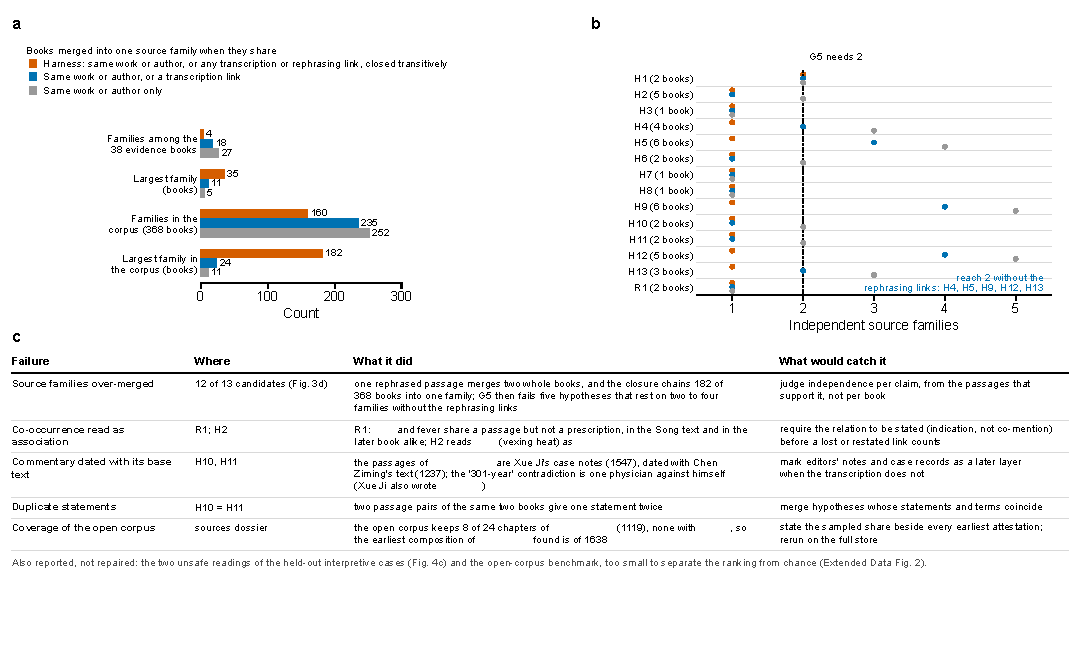
\includegraphics{../../../figures/out/suppfig1_failures.pdf}
\caption{Supplementary Fig. 1}
\end{figure}

\textbf{Supplementary Fig. 1 \textbar{} Where the end-to-end run of Fig.
3 went wrong, and why.} \textbf{a}, Books merged into one source family
under three rules: the harness's (the same work or author, or any
transcription or rephrasing link between their passages, closed
transitively), transcription links only, and the same work or author
only. Under the harness's rule 36 of the 46 books that supplied
evidence, and 233 of the 553 books of the open corpus, fall into one
family. \textbf{b}, The independent families each final hypothesis rests
on under the three rules; dashed line, the two that G5 requires. The
hypotheses that G5 failed and that rest on two to three families once
rephrasing links are left out (H5, H7, H12, H13) include two (H5, H13)
whose evidence is copies of one clause, for which one family is right.
\textbf{c}, The failure modes found by reading every surviving
hypothesis against its evidence, with what each did and the check that
would catch it. None is repaired here: the run is reported as it
happened.

\hypertarget{supplementary-figures-24}{%
\subsection{Supplementary Figures 2--4}\label{supplementary-figures-24}}

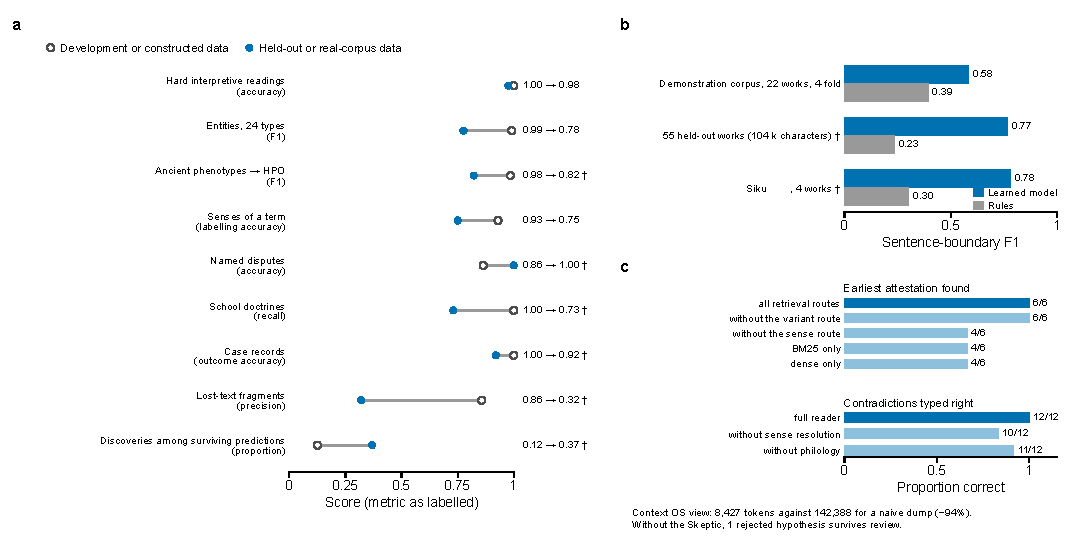
\includegraphics[width=1\textwidth,height=\textheight]{../../../figures/out/extfig1_generalization.pdf}

\textbf{Supplementary Fig. 2 \textbar{} Where the rules transfer and
where they do not.} \textbf{a}, Development or constructed data (open
circles) against held-out or real-corpus data (blue) for nine
capabilities; numbers, the two scores; †, real-corpus value from the
full corpus (\texttt{docs/evals.md}). Development sets were written with
the rules they test. \textbf{b}, Sentence-boundary F1 of the learned
punctuation model and of the rule baseline on the demonstration corpus
(four folds), on 55 works held out of training, and on four unpunctuated
\emph{Siku} texts scored against their JiCheng punctuation (†, full
corpus); every character was preserved in all settings. \textbf{c},
Ablations on the demonstration corpus: earliest-attestation accuracy
with retrieval routes removed (6 terms), contradiction typing without
sense resolution or philology (12 passage pairs), the context supplied
to agents, and review without the Skeptic.

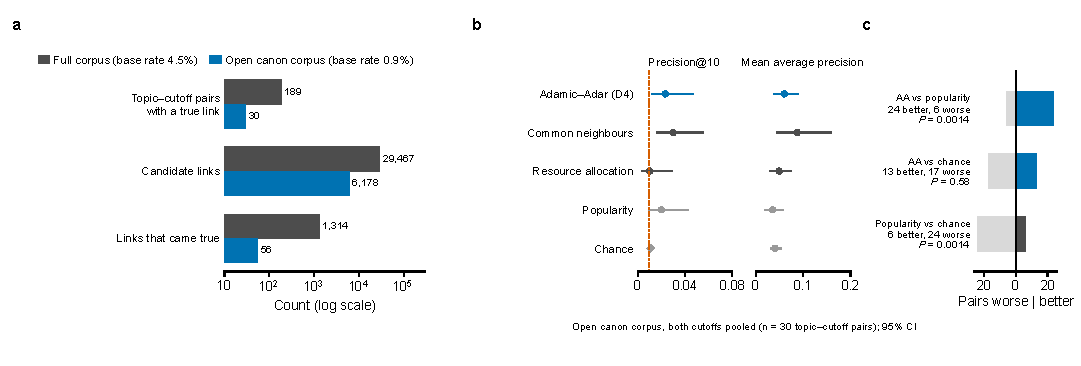
\includegraphics[width=1\textwidth,height=\textheight]{../../../figures/out/extfig2_canon_replication.pdf}

\textbf{Supplementary Fig. 3 \textbar{} The research-value benchmark on
the open canon corpus.} The benchmark of Fig. 5 re-run with identical
rules on the open web corpus (533 works, most sampled by chapters).
\textbf{a}, Average precision of Adamic--Adar (blue), popularity (grey)
and the expectation under chance (open circles) in each of the 51
topic--cutoff pairs in which at least one link came true (24 at 1127, 27
at 1368; log scale); lines join Adamic--Adar to popularity, blue where
Adamic--Adar is higher; right, links that came true in the pair. More
than half of the pairs have a single true link (28 of 51; 109 among
10,115 candidates), so one hit moves a ranking. \textbf{b}, Precision@10
and mean average precision of the five rankers, both cutoffs pooled (n =
51 pairs); dots, means; lines, 95\% confidence intervals; dashed line,
base rate (1.08\%). \textbf{c}, Paired comparisons of average precision,
two-sided sign tests. Adamic--Adar still ranks above popularity (37 of
51 pairs, P = 0.0018) but cannot be told from chance (19 better, 32
worse, P = 0.092), and popularity falls below chance (7 better, 44
worse, P = 1.2 × 10⁻⁷). The benchmark needs the full corpus; the
replication is reported as a limit of the open subset. Every pair and
every prediction: Supplementary Tables 11 and 12.

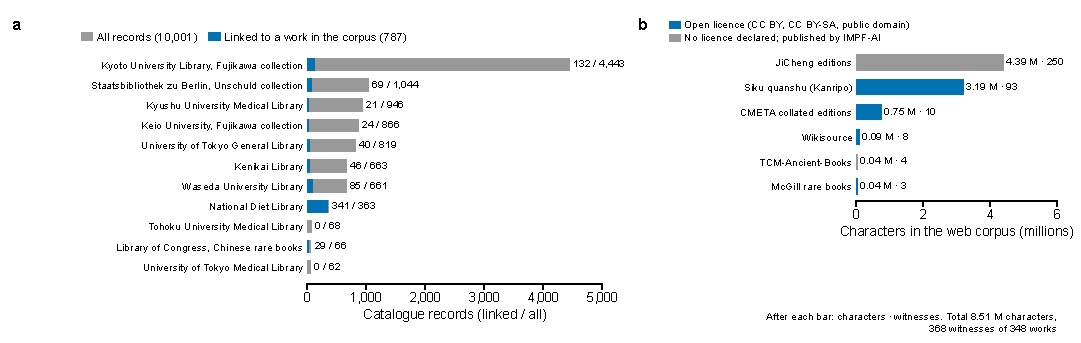
\includegraphics[width=1\textwidth,height=\textheight]{../../../figures/out/extfig3_resources.pdf}

\textbf{Supplementary Fig. 4 \textbar{} The witnesses behind the texts.}
\textbf{a}, Catalogue records of printed and manuscript copies in eleven
digitized collections (title, date, print or manuscript, shelfmark, IIIF
manifest and licence; no image is downloaded) and those linked by title
to a work of the corpus (787 records of 179 works); links made by title
need checking by hand. \textbf{b}, Sources of the open web corpus in
millions of characters and witnesses. Blue, openly licensed
transcriptions: JiCheng, whose selection, arrangement, punctuation and
notes on public-domain texts are released under CC0 1.0 and its own
writing under CC BY 4.0 (the modern editors' part of the few texts it
took from modern reconstructions of lost books excepted); CMETA, CC BY
4.0; Kanseki Repository and Wikisource, CC BY-SA 4.0; McGill, public
domain. Grey, the four TCM-Ancient-Books texts that match no JiCheng
text, whose repository declares no licence, carried on the decision of
the releasing institute (IMPF-AI). Sources whose terms forbid
redistribution are never included. IIIF, International Image
Interoperability Framework.

\hypertarget{supplementary-table-13}{%
\subsection{Supplementary Table 13}\label{supplementary-table-13}}

\textbf{Supplementary Table 13 \textbar{} Sources of the corpus}

\begin{longtable}[]{@{}
  >{\raggedright\arraybackslash}p{(\columnwidth - 8\tabcolsep) * \real{0.2000}}
  >{\raggedright\arraybackslash}p{(\columnwidth - 8\tabcolsep) * \real{0.2000}}
  >{\raggedright\arraybackslash}p{(\columnwidth - 8\tabcolsep) * \real{0.2000}}
  >{\raggedright\arraybackslash}p{(\columnwidth - 8\tabcolsep) * \real{0.2000}}
  >{\raggedright\arraybackslash}p{(\columnwidth - 8\tabcolsep) * \real{0.2000}}@{}}
\toprule\noalign{}
\begin{minipage}[b]{\linewidth}\raggedright
Source
\end{minipage} & \begin{minipage}[b]{\linewidth}\raggedright
Licence
\end{minipage} & \begin{minipage}[b]{\linewidth}\raggedright
Works admitted
\end{minipage} & \begin{minipage}[b]{\linewidth}\raggedright
Characters (millions)
\end{minipage} & \begin{minipage}[b]{\linewidth}\raggedright
Transcription and notes
\end{minipage} \\
\midrule\noalign{}
\endhead
\bottomrule\noalign{}
\endlastfoot
Kanseki Repository KR3e, Siku quanshu medical section (漢籍リポジトリ) &
CC BY-SA 4.0 & 100 & 25.66* & Wenyuange Siku and Sibu congkan
facsimiles; unpunctuated; catalogue with authors, dates, layers \\
JiCheng 笈成 edited texts, v1.4.8 & CC0 1.0 (editorial work); base texts
public domain§ & 816 & 93.64* & Volunteer transcriptions with modern
punctuation; 41 of 857 works excluded \\
CMETA 數位中醫校書郎 collated editions & CC BY 4.0 (collation); base
texts public domain & 11 & 1.49 & Collated page by page against images;
passages carry page numbers and image links \\
Tōa Igaku Kyōkai 東亜医学協会 texts & © the society; local research
only† & 7 & 0.33 & Suwen, Lingshu, Nanjing, Shanghan lun, Jingui yaolüe,
Shennong bencao jing, Bian Que biography \\
Wikisource (Category 中醫, 醫書) & CC BY-SA 4.0 & 18 & 0.77 & Works new
after de-duplication of 627 candidates \\
McGill University Library rare books & Public domain & 5 & 0.40 & Qing
prints and manuscripts on gynaecology \\
TCM-Ancient-Books; tcmoc & Not declared by the repositories‖ & 8 & 0.37
& Mostly simplified copies of JiCheng texts, de-duplicated work by
work \\
Hugging Face classical-tcm-canon & Proprietary-commercial; local
research only† & 1 & 0.31 & One work (Zhang Zhicong's commentary on the
Shanghan lun) \\
Kanseki Repository catalogue (KR-Catalog) & CC BY-SA 4.0 & -- & -- &
Roles and life dates of 132 persons responsible for the Siku works \\
Image catalogues of 11 collections‡ & Recorded per collection & -- & --
& 10,001 records (787 linked to 179 works): title, date, print or
manuscript, shelfmark, IIIF manifest \\
Total & & 966 & ≈123 & 2.05 M passages; 761 distinct works; analysis
periods 475 BCE--1949 \\
\end{longtable}

*Counted in the corpus store (README); the catalogues of these two
sources do not record characters. Other counts sum the catalogue records
of the admitted works.

†Used for local research only and never redistributed; the open web
corpus carries none of the texts whose terms forbid redistribution.

§JiCheng releases its selection, arrangement, punctuation and notes on
public-domain texts under CC0 1.0 and its own writing under CC BY 4.0
(https://jicheng.tw/tcm/copyright.html, consulted 29 September 2026);
the open web corpus carries 427 JiCheng witnesses under these terms,
crediting JiCheng. The modern editors' part of the few texts JiCheng
transcribed from modern reconstructions of lost books is not covered.

‖Mostly simplified-character copies of JiCheng texts; de-duplication
removes every copy, and the 8 texts kept match no JiCheng text. The 4 in
the open web corpus are carried on the decision of the releasing
institute (IMPF-AI); the others are used for local research only.

‡Kyoto University (Fujikawa), Staatsbibliothek zu Berlin (Unschuld),
Kyushu University, Keio University (Fujikawa), University of Tokyo (two
libraries), Kenikai, Waseda University, National Diet Library, Tohoku
University and Library of Congress. Only metadata are held; no image is
downloaded.

Sources are ranked by trust for de-duplication (Kanripo, JiCheng,
McGill, CMETA, AEAM, Wikisource, web collections); a candidate sharing
enough normalized 12-character shingles with an admitted work is
recorded as its copy, while McGill, CMETA and AEAM transcriptions are
kept as independent witnesses. IIIF, International Image
Interoperability Framework.

\hypertarget{supplementary-data}{%
\subsection{Supplementary Data}\label{supplementary-data}}

\textbf{Supplementary Data 1 \textbar{} The Discovery Report of the
end-to-end run}
(\texttt{Supplementary\_Data\_1\_e2e\_discovery\_report.md}): the report
the harness wrote, in Chinese with English section titles, as the
conversation client and the command line show it.

\textbf{Supplementary Data 2 \textbar{} The event log of the end-to-end
run} (\texttt{Supplementary\_Data\_2\_e2e\_event\_log.jsonl.gz}): every
event in order, one JSON object a line, each with its sequence number,
type, actor, principal and payload; replaying it rebuilds the state from
which Fig. 3 and the report were drawn.

\end{document}
